\documentclass[12pt,a4paper,titlepage]{article}


\usepackage{listings}
\usepackage[font={small,stretch=1}, margin=1cm]{caption}
\usepackage{setspace}
\usepackage{graphicx}
\usepackage{geometry}
\usepackage{changepage}
\usepackage{titling}
\usepackage{mathtools}
\usepackage{array}
\usepackage{url}
\usepackage{enumitem}  
\usepackage{subcaption}
\usepackage{algorithm}
\usepackage{amsmath}
\usepackage{algorithm}
\usepackage[noend]{algpseudocode}
\usepackage{xcolor}
\usepackage{tikz}
\usepackage{multirow}
\usepackage[
backend=biber,
style=numeric,
sorting=ynt
]{biblatex}


\makeatletter
\let\OldStatex\Statex
\renewcommand{\Statex}[1][3]{%
	\setlength\@tempdima{\algorithmicindent}%
	\OldStatex\hskip\dimexpr#1\@tempdima\relax}
\makeatother

\definecolor{codegreen}{rgb}{0,0.6,0}
\definecolor{codegray}{rgb}{0.5,0.5,0.5}
\definecolor{codepurple}{rgb}{0.58,0,0.82}

\lstdefinestyle{mystyle}{
	commentstyle=\color{codegreen},
	keywordstyle=\color{blue},
	numberstyle=\tiny\color{codegray},
	stringstyle=\color{codepurple},
	basicstyle=\ttfamily\footnotesize,
	breakatwhitespace=false,         
	breaklines=true,                 
	captionpos=b,                    
	keepspaces=true,                 
	numbers=left,                    
	numbersep=5pt,                  
	showspaces=false,                
	showstringspaces=false,
	showtabs=false,                  
	tabsize=2,
	language=C++,
	basicstyle=\footnotesize,
}

\newenvironment{dedication}
	{\clearpage     
		\section*{Ringraziamenti}      % we want a new page
		\thispagestyle{empty}% no header and footer
		\vspace*{\stretch{1}}% some space at the top 
		\itshape             % the text is in italics
		\raggedleft          % flush to the right margin
	}
	{\par % end the paragraph
		\vspace{\stretch{3}} % space at bottom is three times that at the top
		\clearpage           % finish off the page
	}

\lstset{style=mystyle}

\addbibresource{bibliography.bib}
\linespread{1.5}
\geometry{verbose,tmargin=3cm,bmargin=3cm,lmargin=3cm,rmargin=3cm}

\title{Modularity Based Community Detection on the GPU}
\author{Fontolan Federico}


\begin{document}
	\begin{titlepage}
	\newgeometry{margin=2cm}
	
\includegraphics[width=0.25\textwidth]{0-resources/logo_ca_foscari.png}
   \begin{center}
       \vspace*{2.5cm}
       \textbf{Master’s Degree \\
       	in Computer Science}
 
       \vspace{2.5cm}
       \textbf{Final Thesis}
 
       \vspace{1cm}
		\textbf{\Large\thetitle}
   \end{center}

	\begin{adjustwidth}{0.7cm}{0cm}
		\vspace{5cm}
		\textbf{Supervisor}\\
		Ch. Prof. Claudio Lucchese
		
	
		\vspace{0.5cm}
		\noindent\textbf{Graduand}\\
		Federico Fontolan\\
		Matricolation number 854230
		
		\vspace{0.5cm}
		\noindent\textbf{Academic Year}\\
		2018 / 2019
	\end{adjustwidth}
	
\end{titlepage}
	
	\begin{abstract}
		Modularity based algorithms for the detection of communities are the de facto standard thanks to the fact that they offer the best compromise between efficiency and quality. 
		This is because these algorithms allow analyzing graphs much larger than those that can be analyzed with alternative techniques. Among these, the Louvain algorithm has become extremely popular due to its simplicity, efficiency and precision.
		In this thesis, we present an overview of community detection techniques and we propose two new parallel implementations of the Louvain algorithm written in CUDA and exploitable by Nvidia GPUs, both with a new pruning approach on the input data: the first one is based on the sort-reduce paradigm; the second one is a new hash-based implementation. Experimental analysis conducted on 13 datasets of different sizes ranging from 15 to 150 million edges shows that the both algorithms provide some benefit, but there is not a clear winner. For this reason, we study also an adaptive solution that exploits the best of the two approaches. We compared this algorithm with the two fastest version available: the first is included in the Nvidia project cuGraph; the second in the high performance library Gunrock. Our algorithm performs better in terms of times in the largest graphs. Besides, we optimize the memory consumption: we can analyze graph of almost double size compared to our competitors. 
	\end{abstract}

	\tableofcontents
	\newpage
	\section{Introduction}
The community detection problem is one of the most interesting fields of graph analysis. In several real-world scenarios, we have the necessity of cluster some data considering the relations between them: one example can be the problem of dividing social network users in groups by the mutual friendship relations to propose targeted advertisings. A natural way to represent this kind of structure based on the relation is a graph, and several techniques based on this theory was proposed in the literature to solve this kind of problem. This problem is not easy to solve due to the extremely high number of different possible partitions of the data that we can perform, even if the dataset is composed of few elements.
One the most famous and used heuristic is the Louvain algorithm proposed by Blondel et al. \cite{Blondel_2008}, due to its speed and its overall quality, even if its limits are well known in the literature. This greedy algorithm divides the graph into partitions maximizing a quality function that evaluate them, called \textbf{modularity}. This function is based on the idea that a random graph doesn't exhibit a community structure: therefore, we can evaluate how is well defined the community structure comparing the graph with another graph that keeps some of its structural proprieties but is generated at random, called \textit{null-model} \cite{Girvan2002Community}. Given a graph $G(V,E)$, its adjacency matrix $A$, a partition of nodes $C$ and the corresponding function $c(x)$ that assign each node $x$ to its community, we define the modularity function as follow:
\begin{equation}\label{intro_Q}
Q = \frac{1}{2|E|} \sum_{i,j \in V}\left(A_{ij} - \frac{k_ik_j}{2|E|}\right) \delta(c(i), c(j))
\end{equation}
where $k_i$ is the degree of the node $i$ and $\delta$ is an filter function: its yields one if $c(i) = c(j)$, zero otherwise.
The techniques proposed before the Louvain algorithm are quite slow because, every time we assign a node to a community, we have to recalculate the values with the previous formula, and this calculation takes a lot of time. To speed up the computation, this algorithm proposed to calculate the variation in modularity assigning a node to another community without recalculating $Q$ with the Formula \ref{intro_Q}. The algorithm is composed of two phases: an optimization phase and an aggregation phase. At the beginning each node is assigned to a community composed only by itself; in the first, we pick each node $i$ of the graph and we calculate for each community $c_j$ in its neighbourhood the values $\Delta Q_{i \rightarrow c_j}$, that is the changing in the modularity of assigning the node $i$ to the community $c_j$, as following:
\begin{equation}\label{intro_Delta}
\Delta Q_{i \rightarrow c_j} = \frac{l_{i\rightarrow c_j} - l_{i\rightarrow c_i / \{i\}}}{2|V|} + k_i \frac{k_{c_i / \{i\}} - k_{c_j}}{4|V|^2}
\end{equation}
where $l_{i\rightarrow c_j}$ is the sum of edges that connect $i$ to the community $c_j$, $k_i$ is the weight of the nodes $i$ and $k_{c_j}$ is the weight of the community $c_j$. Then, for each node, we select the maximum values and if it is greater than zero, we assign the node $i$ to the community that corresponds to the maximum value. We repeat this procedure sequentially for all nodes while the modularity score increases. When no more improvement can be achieved, we execute the aggregation phase. In this phases we create a new graph from the current community structure: each node is one of this communities, and the edge between them is given by the sum of the links between nodes that belong to the corresponding communities (edge between nodes in the same communities lead to self-loop). After this step, we reapply the first step. The algorithm ends up when no more improvement is obtained.
This algorithm is quite efficient with a complexity of $O(m)$ where $m$ is the number of edges in the graph, but this algorithm requires a lot of time to find the communities in the bigger graphs. For this reason, some approaches were proposed in the literature to speed up the algorithm. One interesting technique proposed by Ozaki et. al \cite{pruning}, prune the nodes in the optimization phase, considering only the nodes that have a neighbour that has to change its community in the previous iteration. Apart from this kind technique, generally, the most effective method to improve significantly the performance of an algorithm is to parallelize the execution. Especially, to obtain the maximum speed, many frameworks that allow performing on the GPU computation normally handled by the CPU became popular. The most used framework is the Nvidia CUDA, a parallel computing platform and application programming interface. CUDA was originally designed as a C++ language extension that allows any developer to building application designed for the GPU with a low learning curve. CUDA is also designed to transparently scale on different GPU.\\
In literature, several implementations of the Louvain algorithm for the GPU were proposed. In this thesis, we present three new algorithms for the GPU based on the Louvain algorithm: PSR-Louvain, PH-Louvain and Adaptive Louvain. All these algorithms implement the pruning techniques proposed by Ozaki. No other Louvain based algorithm for the GPU implements this technique before. 
These algorithms compute the maximum score of $\Delta Q$ for each node simultaneously, and then we update the community based on that score. Also, the creation of the edges of the new graph in the aggregation phase is executed in parallel. 
The first two algorithms are quite similar to each other. In both algorithm we start from the edge list composed by the tuple $(i,j,w)$ where $i$ is the source node of the edge, $j$ is the destination node of the edge and $w$ is the weight of the edge.
Both algorithm, in the optimization phase, first select only the edges such that the node $i$ has a neighbour that has to change its community in the previous iteration, then they substitute each destination node with the corresponding community $c_j$. After them, the two algorithms using different methods to sum up all the values $w$ for each pair $i$ and $c_j$ and obtain the corresponding $l_{i\rightarrow c_j}$. We need this value to compute all the $\Delta Q_{i \rightarrow c_j}$, as shown in the Formula \ref{intro_Delta}. The first algorithm sorts the list and then performs a segmented reduction to each value with the same pair $i$ and $c_j$; the second algorithm use a hashmap to aggregate all of these values. After then, both select the maximum value for each node and eventually update the community. Finally, they compute if a node has a neighbour that change its community and store the results that will be used in the next iteration for the pruning. These two algorithms use the same aggregation scheme proposed in the optimization phase to create the new graph in the aggregation phase. In both algorithm is also present a technique that optimizes the first iteration of each optimization phase. \\
This two algorithm, compared to the fastest sequential versions, obtain a speed-up factor up to 56.
During the analysis of this two algorithm, we discover that the PSR-Louvain tends to perform better than the PH-Louvain in the early iteration of the optimization phase; on the other hand, the PH-Louvain approach outperforms the other when the number of a different key inserted in the hashmap falls below a given threshold. Besides the PH-Louvain aggregation phase is faster than the PSR-Louvain one. \\
On these considerations, we create a new algorithm that combines these two algorithms and selects the best aggregation scheme on the situation. This Adaptive approach performs better than the other, combining effectively the best feature of these two algorithms. Finally, we compare this version with the two fastest GPU Louvain based algorithm: the first one is included in the Nvidia library cuGraph; the second one is included in the high-performance library for graph analysis Gunrock. Our test highlight that our Adaptive algorithm optimizes the memory occupation better than the other two allowing it to compute graph with approximately twice edges. Besides, our algorithm generally perform better than these two algorithms in terms of time.\\
This thesis is structured as follows:
in Chapter \ref{C2} of this thesis, we present the Nvidia GPUs architecture and the CUDA framework, paying special attention to the concept that is used later on this thesis; in the Chapter \ref{C3} we present the field of the community detection and the modularity optimization, highlighting the motivation that leads to the design of the Louvain Algorithm; in the Chapter \ref{C4} we present the sequential Louvain algorithm, the pruning techniques and the previous parallel implementations presented in the literature;
then, in Chapter \ref{GPUalg}, we present in details our two first algorithm, that will be analyzed in details in the Chapter \ref{C6}; finally, in the Chapter \ref{C7}, we present the Adaptive Louvain algorithm and we analyze it, comparing it first with our other two algorithms, then with the two algorithms included in the two libraries. In the last chapter, we sum up our work and we highlight some future research areas and development.
	\newpage
	\section{Nvidia GPUs architecture and CUDA}
The scientists, years by years, have to face bigger and bigger problems. 
Even if Moore's law (that said: "the number of transistors in an integrated circuit double about every two years") determines the increased power of the CPU since the sixties, even the problems size grows and it grows also much more quickly. For example, the web growth since the turn of the millennium raises new challenges that are hard to solve with the standard algorithm, due to the size of the data.  \\
Besides, at the same time, the manufacturers have to face some serious physical limits. The increase in performance was made possible by the reduction in the size of the transistors and the increase in the frequency of the clock cycle. In the first half of the two-thousands, the producers discovered that reducing, even more, the size cause serious problems of heat dissipation and data synchronization. To find a solution to this problems, the manufactures start to produce multi-core CPU: the idea is that if it's impossible to increase further the speed with only one core, they add another processing unit, to ideally halve the execution time.\\
For these reasons, in recent times the studies of new parallel approaches became fundamental to solve problems that can not be solved classically. As a result of this change and at the same time both the support of floating-point number on the graphics processing units (GPU) and the advent of programmable shaders, it became popular the general-purpose computing on GPU (GPGPU), i.e. the use of a GPU to perform a computation that is commonly handled by the CPU.\\
\begin{figure}[h]
	\centering
	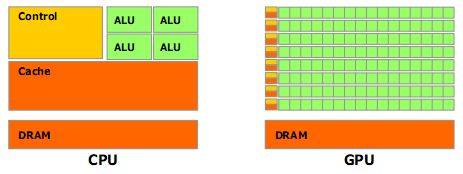
\includegraphics[width=0.7\linewidth]{0-resources/cpugpuhardware}
	\caption{Difference in CPUs and GPUs architecture. This image was reprinted from \cite{cuda_manual} }
	\label{fig:cpugpuhardware}
\end{figure}
\\
The GPU architecture is radically different respect to the CPU. The CPU has several ALUs (Arithmetic and Logic Unit), a complex control unit that controls those ALUs, big fast cache memory and dynamic random access memory (DRAM); the GPU has many ALUs, several simple control units, a smaller cache and a DRAM (Figure \ref{fig:cpugpuhardware}). While the first one is focused on the low-latency, the second one is focused on the high throughput;
while the first one is focused on handle various serial complex instruction, the second is focused on handle much parallel simple instruction.
In brief, the first one is a versatile processing unit, the second one is highly specialized.
Even if in recent time the multi-core CPU performance get closer to the performance of the GPU \cite{gpucpu}, from the Figure \ref{fig:cpugpu} we can see how the performance of the GPU outclasses the performance on the CPU.\\
\begin{figure}[h]
	\centering
	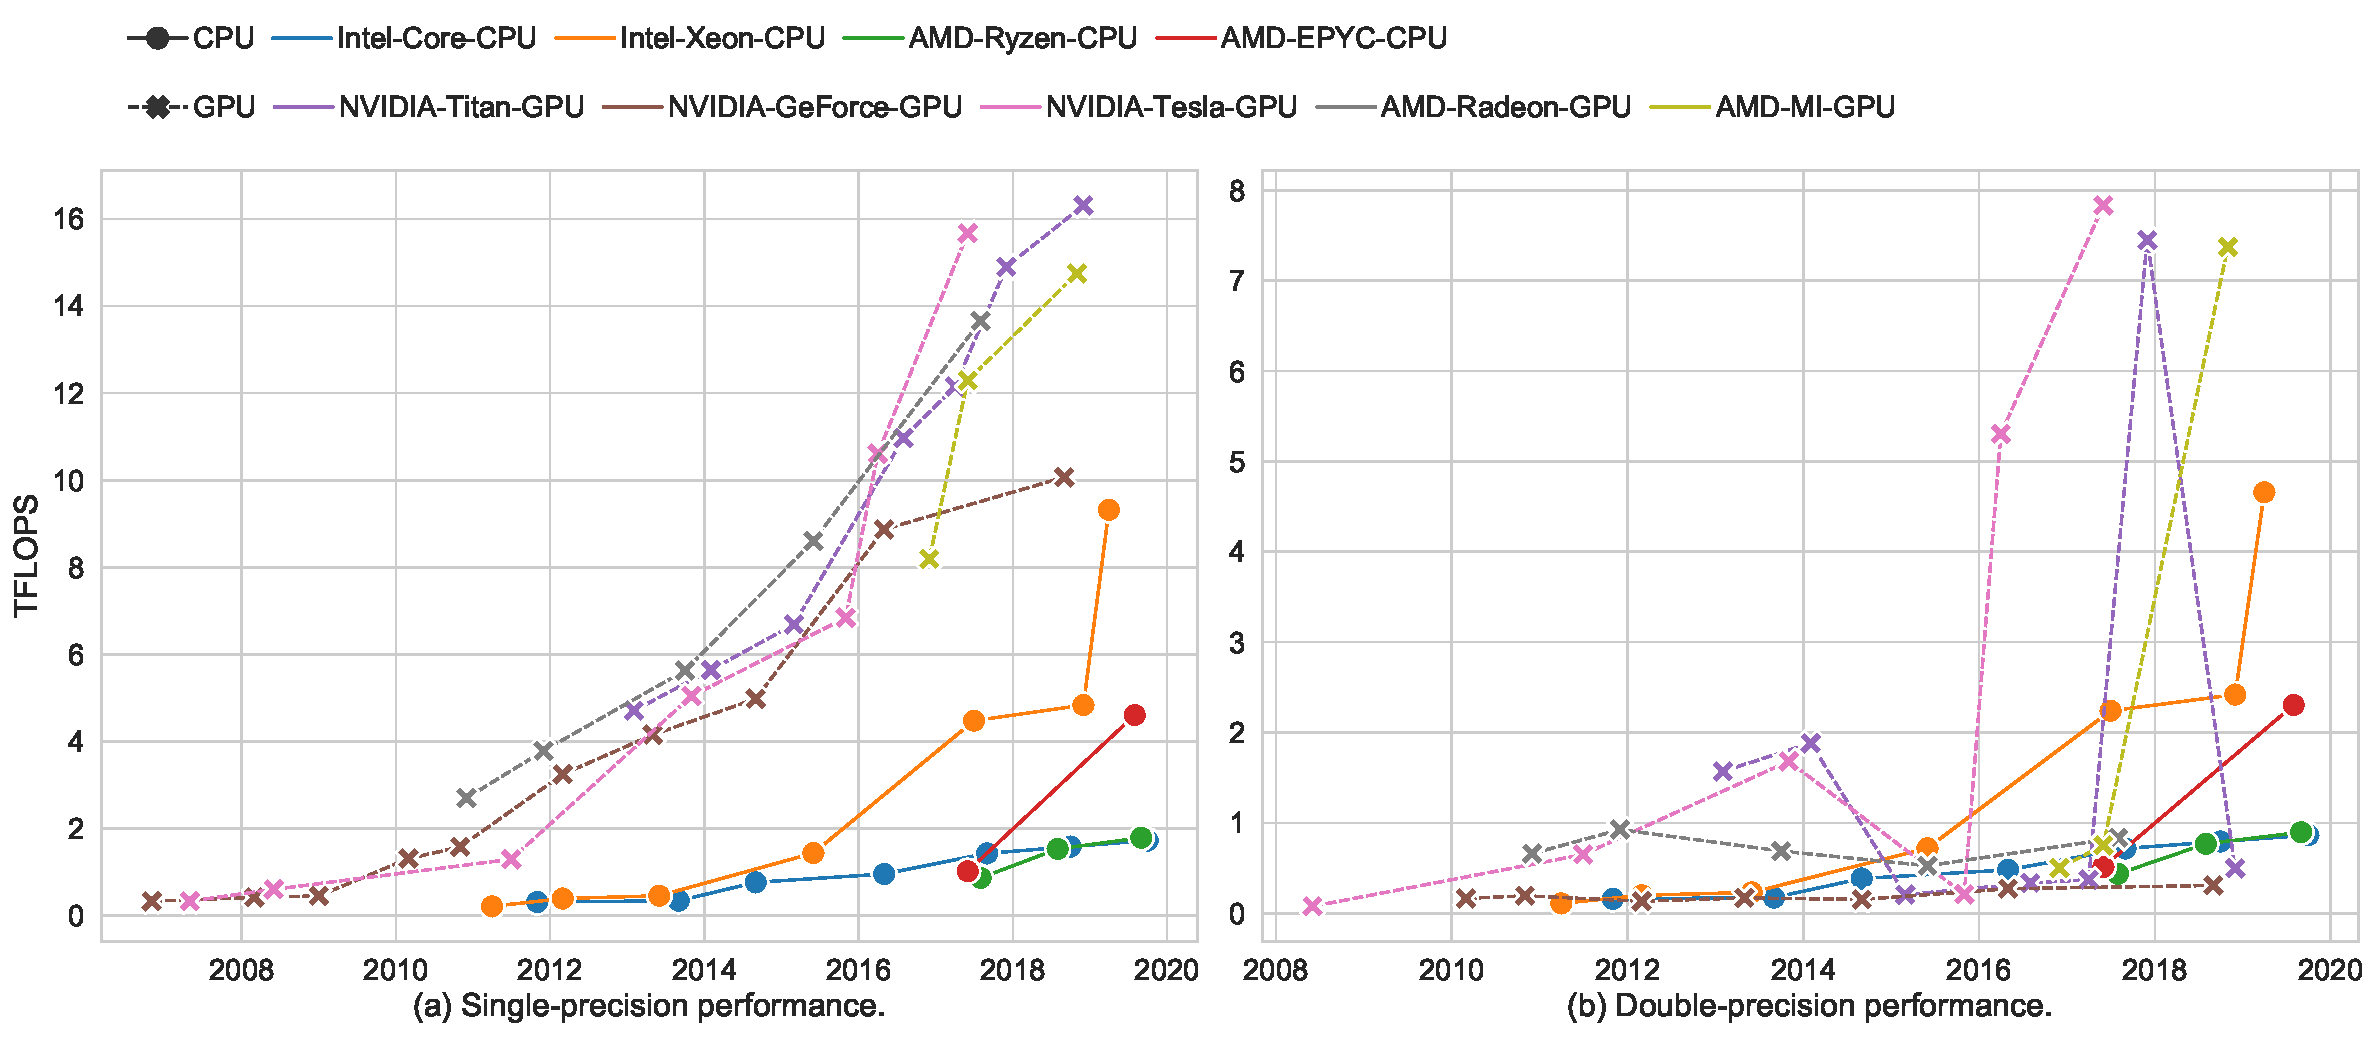
\includegraphics[width=1.\linewidth]{0-resources/cpu_gpu}
	\caption{Comparing single-precision and double-precision performance of CPUs and GPUs. The performance are measured in trillion of floating point operations per Second (TFLOPS). This image was reprinted from \cite{gpucpu}.}
	\label{fig:cpugpu}
\end{figure} 
\\	
For those reasons, the GPU-accelerated applications are the most effective to solve big problems, due to the possibility of reach very high speed-up compared to the classic multi-core applications. 
To simplify the development of this type of applications, in 2007, Nvidia releases CUDA (Compute Unified Device Architecture), a parallel computing platform and application programming interface (API) model.
Nowadays, the CUDA framework is one of the main tools to develop HPC applications, due to its performance and simple API, and for this, we choose to use it in this project.
In this chapter, first of all, we present the Nvidia's GPU architecture,  then after we present CUDA basis and Thrust, a library that was used in the project presented in this thesis that simplifies the development. This chapter was based on \cite{turing} and \cite{cuda_manual}.
\subsection{Nvidia's GPU Architecture}
Now we present Nvidia's GPU Architecture to introduce some key concept that is used later in the thesis. This introduction present the last architecture released by Nvidia, Turing. We present the highest performing GPU of the Turing line, The Turing TU102 GPU (Turing machine can be also scaled down to the scaled-down from this one). 
In Figure (\ref{fig:tuning:a}) we can see a scheme of this architecture.
\begin{figure}[h]\label{fig:tuning}
	\hspace*{-4em}
	\subcaptionbox{\label{fig:tuning:a}}{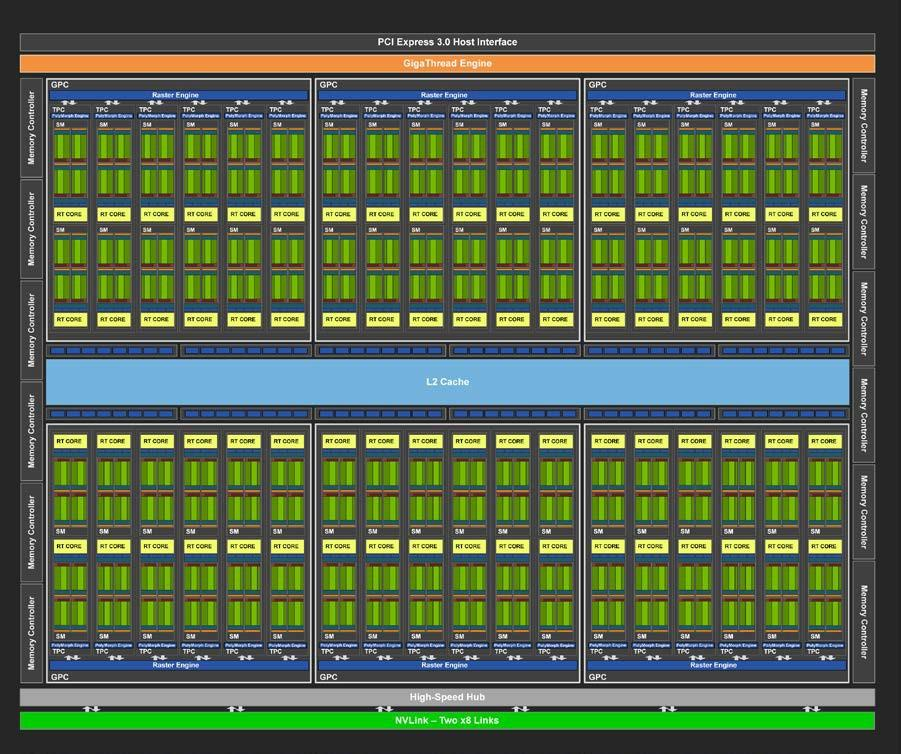
\includegraphics[width=0.72\linewidth]{0-resources/turing}}\hspace{4em}%
	\subcaptionbox{\label{fig:tuning:b}}{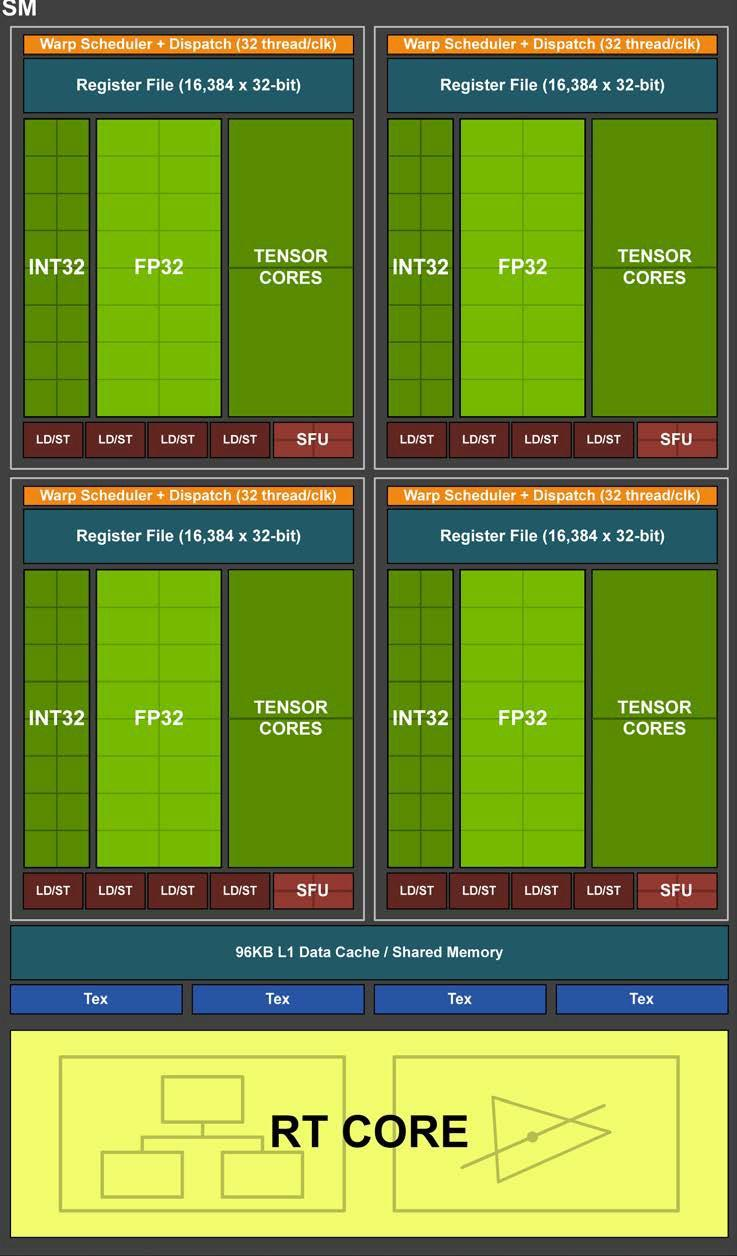
\includegraphics[width=0.4\linewidth]{0-resources/sm}}
	\caption{(a): Tuning GPU full architecture; (b) Streaming multiprocessor (SM) in details. Those images was reprinted from \cite{turing} }
\end{figure}
The cornerstone of each Nvidia's GPU is the concept of Streaming Multiprocessor (SM), that are represented in Figure (\ref{fig:tuning:b}): it contains some cores specialised to solve specific arithmetic operations on specific types of data (like integer, float, double, tensor...).
In a Tuning machine, each SM contains 64 FP32 cores, 64 INT32 cores, eight Tensor cores and two FP64 cores (that aren't present in Figure \ref{fig:tuning:b}). In tuning architecture is present also a Ray Tracing cores in each SMs: this core is used in rendering.\\
The SM is the fundamental unit because, as we see soon, the parallel execution of the code in a CUDA application it's organized in blocks, and each block is executed on a single SM. 
Moreover, the SM contains also some register (256 KB in Turing), an L1 cache and a shared memory (in Turing 96 KB of L1/shared memory which can be configured for various capacities). 
The multiprocessor creates, manages, schedules, and executes threads in groups of
32 parallel threads called warps: when a multiprocessor is given one or more thread blocks to execute, it partitions them into warps that get scheduled by a warp scheduler for execution. 
A very important notion is that each warp executes one common instruction at a time, so if threads of a warp diverge via a conditional branch, the warp serially executes each branch path taken, ignoring the instruction for the threads that are not on the active path. 
The registers are private for each thread, but all threads share the SM's shared memory.\\
The SMs are organised in Texture Processing Clusters (TPCs), that in a Turing GPU contains two SMs.
In their turn, the TPCs are organized in Graphics Processing Clusters (GPC) that in a TU102 contains six TPCs. Finally, each GPU's contain six GPCs. Shared to all component there is an L2 cache: this is used as global memory, i.e. each thread can have access to it. In the Turing GPU. it is large 6144 KB.
Therefore, in summary, a Turing TU102 GPU contains 72 SMs and than 4608 FP32 cores, 4608 INT32 cores, 576 tensor core and 144 FP64 cores.

\subsection{CUDA}
In November 2006, CUDA (that stands for Compute Unified Device Architecture) was realised by NVIDIA. This general-purpose parallel computing platform aims to give a framework to the developers that allow building applications that transparently scale its parallelism with a low learning curve. To overcome this challenge, CUDA was designed as a C++ language extension: in this way, a programmer that already know the language syntax can start to develop a GPU-accelerated application with a minimal effort. The support of other language was introduced years by years, as illustrated in Figure \ref{fig:gpu-computing-applications}. In this chapter we present the C++ extension, that was used to develop the project illustrated in this thesis, even if all extensions share the same concept and programming model.
\begin{figure}
	\centering
	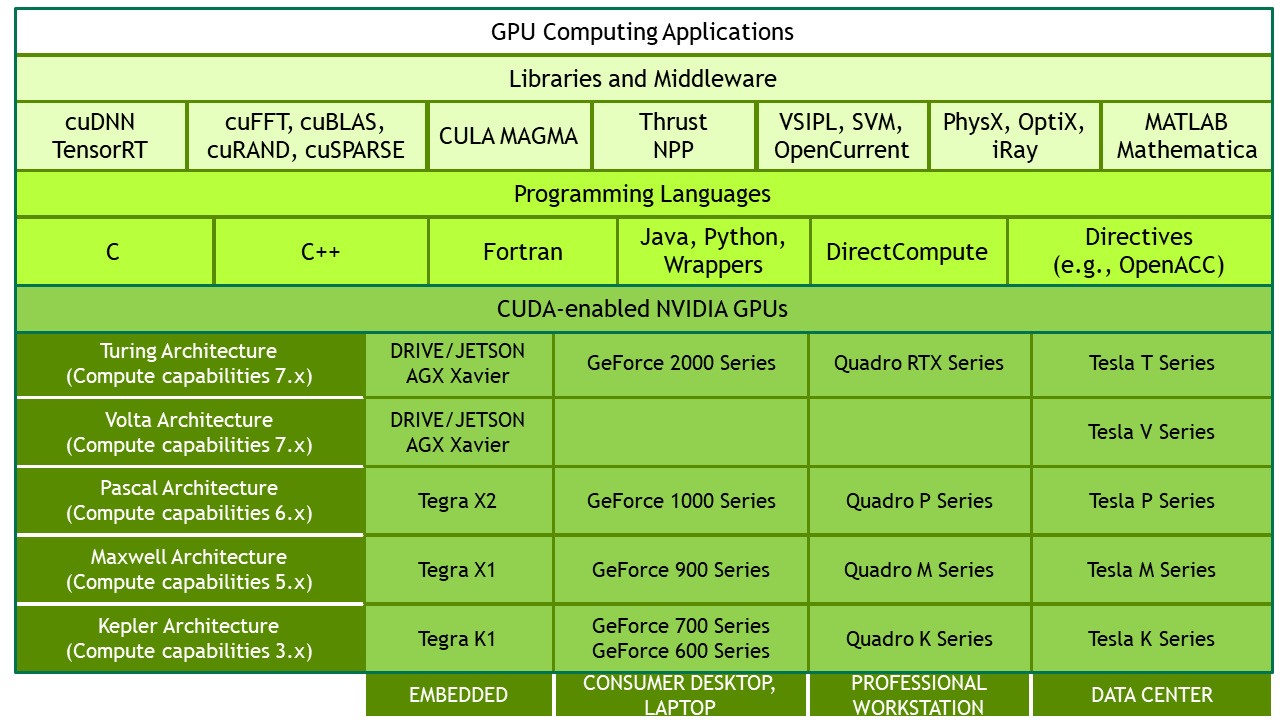
\includegraphics[width=0.8\linewidth]{0-resources/gpu-computing-applications}
	\caption{GPU Computing Applications. This image was reprinted from \cite{cuda_manual}.}
	\label{fig:gpu-computing-applications}
\end{figure}\\
The first key concept is the \textbf{kernel} function. In a CUDA-based application we define as \textbf{device} the GPU and as \textbf{host} the CPU. The application starts to the host, and when it is needed, it calls a kernel function that executes the function N times in parallel by N different threads. To define a kernel, we have to add \verb|__global__| declaration specifier to the method and the number of thread that have to execute the kernel call. Each thread has a unique ID. To set this number we use an execution configuration syntax: after the method name, we include this setup enclosed in three angle brackets \verb|<<< ... >>>|. The configuration is used to define the number and sizes of the blocks: a block is a group of threads that are organized in a one, two or three dimensional way. To identify the threads referring to the block, they have the three-component vector \verb|threadIdx| that identify its position.
In their turn, also the blocks are organized into a one-dimensional, two-dimensional or three-dimensional grid. Similar to the previous one, the vector \verb|blockIdx| identify the block into the grid, and each thread can see each owns. To define the dimensions of the grids and the blocks in the angle brackets, we use two \verb|dim3| (or eventually \verb|int| to define a one dimension grid/blocks). The total number of threads is equal to the number of threads per block times the number of blocks: using the same logic, we can recover the unique ID of the vector from \verb|threadIdx| and \verb|blockIdx|. In Figure \ref{fig:blocks:a} is illustrated the grid-blocks schema.
\begin{figure}
	\hspace*{-4em}
	\subcaptionbox{\label{fig:blocks:a}}{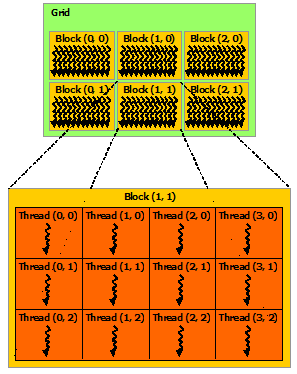
\includegraphics[width=0.5\linewidth]{0-resources/grid-of-thread-blocks}}\hspace{1em}%
	\subcaptionbox{\label{fig:blocks:b}}{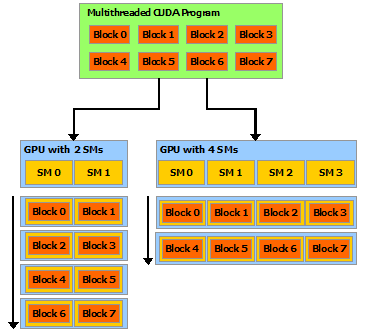
\includegraphics[width=0.7\linewidth]{0-resources/automatic-scalability}}
	\caption{(a): Grid of Thread Blocks; (b) Automatic Scalability. Those images was reprinted from \cite{cuda_manual} }
\end{figure}\\
As mentioned above, each block is assigned to a different streaming multiprocessor. On current GPUs, a block has threads limit set to 1024, due to the limited memory resources of the SM. This block scheme is used to implement automatic scalability: indeed, the GPU schedule each block thread on any available SM, in any order. For example, if we have a program that divides the threads into eight blocks, it can be executed from both two GPU's with respectively two and four SMs without any intervention on the scheduling from the developer (Figure \ref{fig:blocks:b}).
\begin{figure}
	\centering
	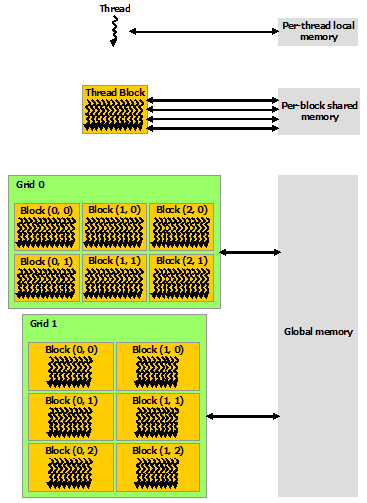
\includegraphics[width=0.52\linewidth]{0-resources/memory-hierarchy}
	\caption{Memory Hierarchy. This image was reprinted from \cite{cuda_manual}.}
	\label{fig:memory-hierarchy}
\end{figure}
By other hands, the block schema allows also threads collaboration: as illustrated in the Figure \ref{fig:memory-hierarchy}, thanks to the allocation of each block to the same SM, allows those threads to share a fast per-blocks memory. Besides, all threads share the global device memory, even if they belong to different blocks or kernel (some advanced settings permit to execute two kernels simultaneously if there are enough resources. Those settings are not presented here because there aren't used in this thesis because a large amount of data doesn't permit to parallelize those kernels. Moreover, for the sake of completeness, they are well described in \cite{cuda_manual}). The data must be copied to this memory from the host before the kernel execution. Those two type of memory, combined to several primitives that synchronize thread at warp, blocks or device levels, permitting threads collaboration. Those synchronizing function acting as a barrier: all threads in the specific level must wait for the others before any is allowed to proceed. In addition, CUDA exposes some other primitives that allow atomic operations: if multiple threads call one of those methods on a specific memory address, the access to it will be serialized. No information about the order of the operation will be given a priori.
In conclusion, we remark that every new hardware architecture could introduce new features that aren't supported by the old GPU. For this reason, CUDA uses the concept of Compute Capability to identify the features supported by the GPU hardware. 

\subsection{Thrust Library}
To conclude this CUDA introduction, we present Thrust, a powerful library of parallel algorithms and data structures that are largely used in this thesis project. This C++ Standard Template-based library is included in the CUDA toolkit and provides a reach collection data-parallel primitives (as transform, sort or reduce) that allows writing a high performing and readable code with minimal effort. This presentation is based on the Thrust section present in the CUDA manual \cite{cuda_manual}.\\
We start the presentation from the two vector containers, \verb|host_vector| and \verb|device_vector|. As their name says, they are arrays that are dynamically allocated respectively in the host and the device memory. Like the \verb|std::vector|, they are generic containers, their elements are allocated in contiguous storage locations and they can dynamically change the size. Indeed, using the \verb|=| operator, we can copy a \verb|host_vector| in a \verb|device_vector| and vice-versa. 
Thrust also provides many useful parallel algorithms, implemented for both host and device, like:
\begin{itemize}
	\item Sort that performs the sorting of a vector. It is also present its "by key" version that sorts a vector of values using another vector as a key;
	\item Reduce that performs a reduction of a vector. It is also present its "by key" version that, given a vector of values and a vector of keys, performs a reduction of the values for each consecutive group of keys;
	\item Transform that applies a function to each element of the vector;
	\item Exclusive and Inclusive Scans that perform a prefix sum, respectively ignoring and considering the corresponding input operand in the partial sum.
\end{itemize}
In this thesis, we use only the device CUDA-based version of this algorithm.
The last useful feature that Thrust provides is the fancy iterators. These iterators are used to improve performance in various situations. The \verb|transform_iterator|, for example, were used to optimize the code performing the transformation during the execution of an algorithm. Another very useful iterator is the \verb|zip_iterator| that takes multiple input sequences and yields a sequence of tuples: in this way we can treat many vectors as a single one and perform more operations simultaneously.
	\newpage
	\section{Community Detection State of the Art}
\begin{figure}[h]
	\centering
	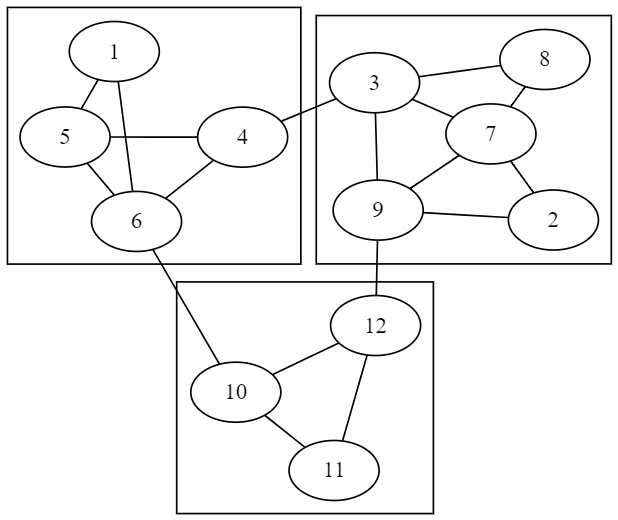
\includegraphics[width=0.6\linewidth]{0-resources/community1}
	\caption{An example of a communities structured graph. In it is well visible three community, enclosed by the rectangles. The image was made with Graphviz.}
	\label{fig:community1}
\end{figure}
The problem of community detection raises in many application scenarios from the necessity of finding groups of objects that have a large number of connections to each other. To represent problems where it is fundamental to empathize connection between objects, the graph theory is the main tool. A graph is a mathematical structure composed of nodes (or vertices) that denote the objects and edges (or links) that express some kind of relationship between objects and possibly having a weights that quantifies this relationship.
The Graph Theory born in 1736 when Euler used this mathematical abstraction to solve the puzzle of Königsberg’s bridges. Since then, this tool was used in several of Mathematics, Social, Biological and Technological application. In recent time, the approach to this studies has been revolutionized to deal with bigger and more complicated challenges, supported by the increasing computing power.
\begin{figure}[h]
	\centering
	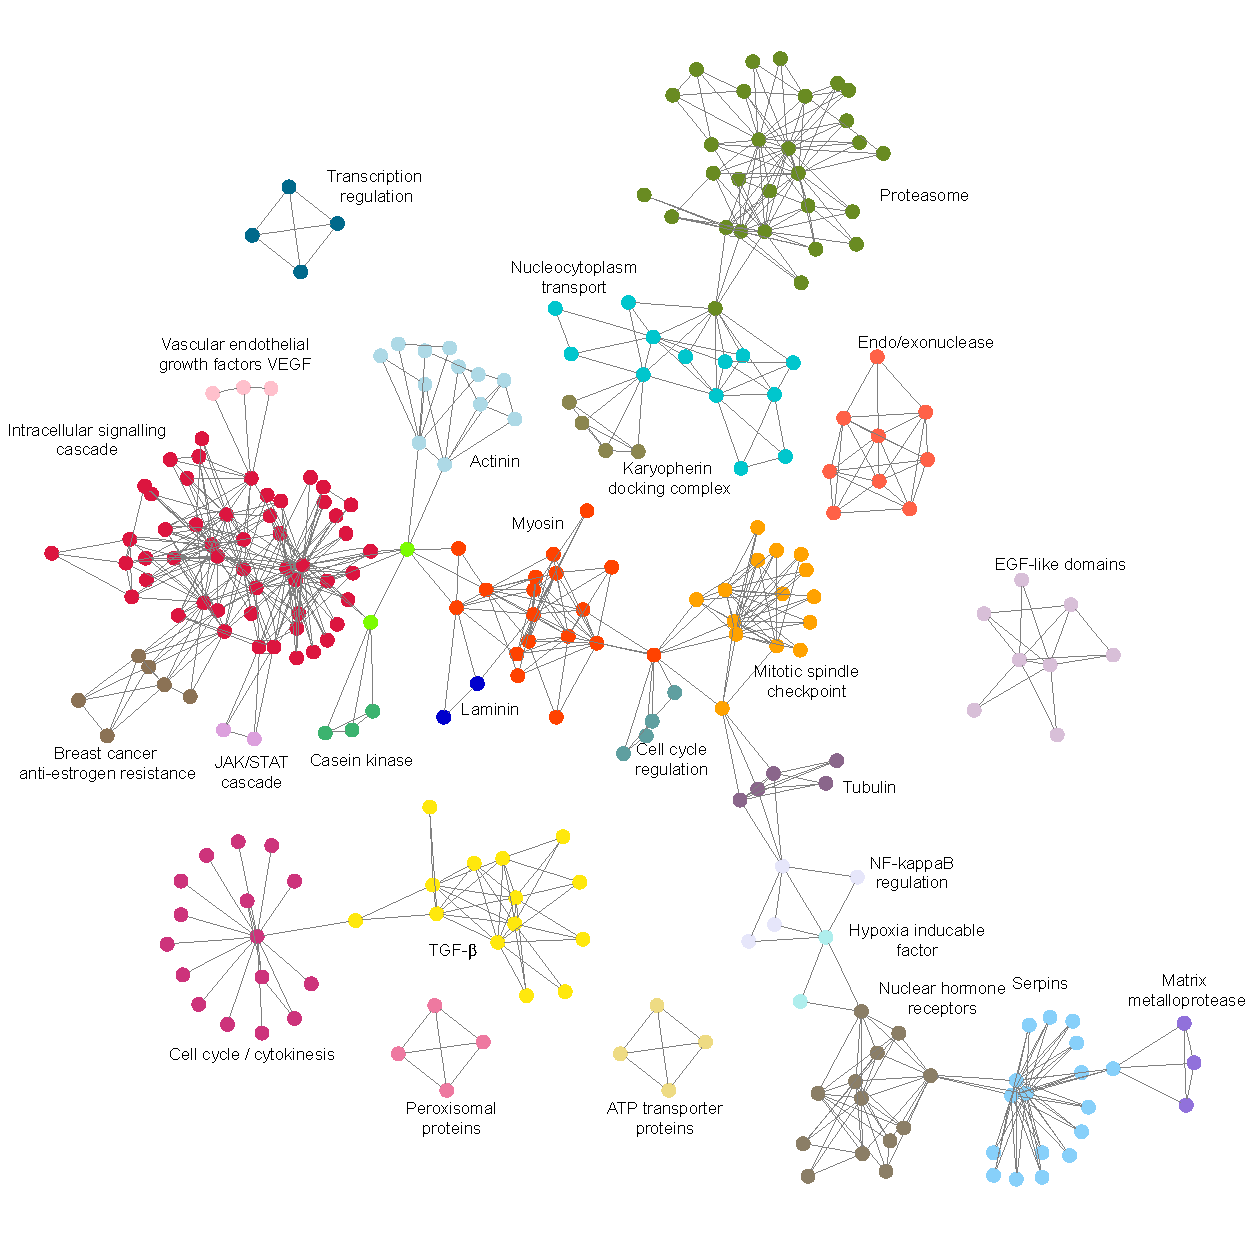
\includegraphics[width=1\linewidth]{0-resources/ppi}
	\caption{A protein protein iteration network of a rat cancerous cell. This image was reprinted from \cite{metastasis}.}
	\label{fig:ppi}
\end{figure}\\
The necessity of finding this high-connected substructure in graph arises from real problems of the previous field: for example, the study of Protein-Protein Interaction (PPI) networks is very important because the interaction between proteins is the basis of all process in the cell.\\ A study demonstrated that this type of network shown to be useful for highlighting key proteins involved in metastasis. \cite{metastasis} \\
Other examples can be found in the field of sociology: a historically well-know scenario is the Zachary's Karate Club. This dataset captures members of a Karate Club for 3 years.\cite{Zac77} An edge between two nodes represents an interaction between two members outside the club. At some point, a conflict between the administrator and a master led to split of the club into two separate groups. The question is if it is possible to infer who compose these two new groups basing on the information that this graph give to us. 
\begin{figure}
	\centering
	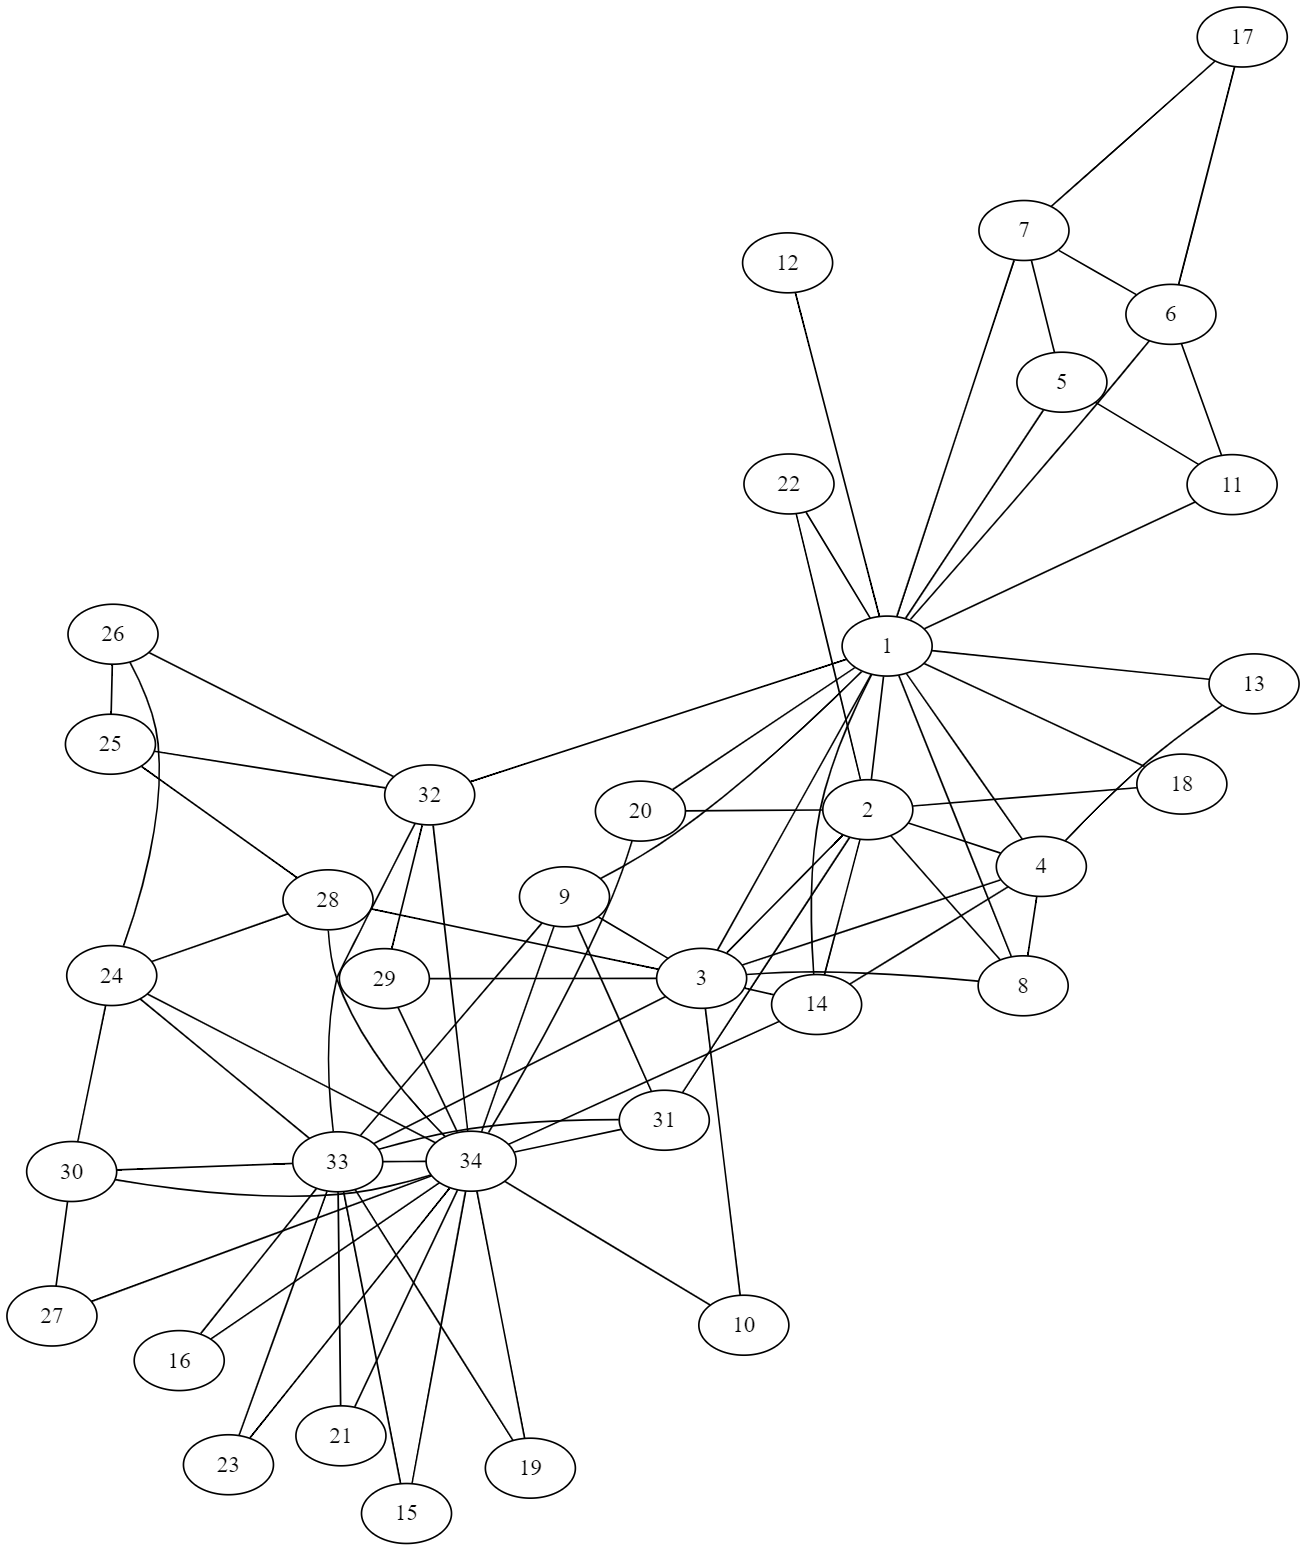
\includegraphics[width=0.6\linewidth]{0-resources/karateclub}
	\caption{Zacahry's karate club. \cite{Zac77} This image was made with Graphviz.}
	\label{fig:karateclub}
\end{figure}
This small network of 1977 is famous because it has often been used as a reference point to test the detection algorithms used to analyze huge social web networks.
In general this kind of problem, i.e. clustering people that belong to the same community base on interaction, it's useful not only in sociology but also in marketing: by knowing people with similar interests, it's possible to make better recommendation systems.\\
There are several of similar scenarios to apply this method in the real-world, all united by the fact that the data are unregular but it's present some well-defined topological structure that in a completely random graph are absent. A random graph is a fully disordered graph, firstly proposed by Erdös and Rényi \cite{random} in 1959: it's a graph where the probability that there is an edge between two nodes it's equal for all pairs of nodes and, for this reason, the degree of the nodes (i.e. the number of edges incident to a node) is homogeneous. In real networks, this is not true, because they are often scale-free (fallow a power-law distribution). An example of this is the study about the citations in scientific papers made by Derek J. de Solla Price in 1965 \cite{dsp} or the study about World Wide Web growing made by Albert-László Barabási et al in 1999 \cite{Barab}.
Furthermore, the degree distribution of the nodes is non-homogeneous not only globally but also locally, this due to the observation that there is a high concentration of edges within sets of nodes and a low concentration of edges between this sets. These two concepts are essential to formulate the formal definition of Community and Modularity. In this chapter will be presented some definitions of community and will be given an overview of some methods that are used to identify communities.
\subsection{Community Definitions}
The informal definition of community is there are many more edges inside the community versus the rest of the graph, but there isn't a unique quantitative definition of community. This kind of freedom is necessary because the concept of community is strictly connected to the problem that will be analyzed: for example, in some cases, it's necessary that community overlap, but in other problems, this is not necessary. There is a unique key constraint that allows talking about community detection: the graph must be sparse. A sparse graph is a graph where the number of nodes has the same magnitude of the number of edges. In the unweighted graph case, if the number of edges is far greater than the number of nodes, the distribution of edges among the nodes is too homogeneous for communities to make sense \cite{fortunato}. In that case, the problem nature is little different: we aren't interested anymore on the edge density between nodes but we have to use some kind of metrics (like similarity or distance) to clustering. In that case, the problem is more similar to data clustering. Despite this, assuming that a community is a subset of similar nodes it's reasonable, for this reasons some techniques (like spectral o hierarchical clustering) belonging to this field are adopted in community detection and will be shortly presented later on this thesis.
Following this, Fortunato \cite{fortunato} defines three main classes of community's definitions: \textit{local, global and based on vertex similarity}. Other types of definitions are still possible, but these three offers give a good summary of the problem. Now those classes will be presented to give an overview of the various approach that has been used to define this problem. 
\subsubsection{Local definitions}\label{local-def}
Considering that a community has a lot of interactions with the other nodes that are in it and few connections outside, it is fair to think about the communities as autonomous objects.
The local definitions are based on this concept. Directly from this concept, we can think at the community as a clique, i.e. a subset whose vertices are all adjacent to each other. This type of definitions it's too strict: even if just one edge is not present, the subset is not a clique, but the subset has a very high concentration of edges. For this reason, the clique definition is often relaxed, using, for example, $n$-clique, i.e. a subset in which all the vertices are connected by a path of length less than $n$.\\
Anyway, this type of definitions ensure that there is a strong cohesion between the nodes in the subset, but not ensure that there isn't a comparable cohesion between the subset and the rest of the graph. For this purpose, other definitions were proposed. 
Given a graph $G(V,E)$, the relative adjacency matrix $A$ and a subset of nodes $C$ where $C \in V$, we define the internal degree $k_v^{int}$ and the external degree $k_v^{ext}$ for each vertex $v$ that belongs to $C$ as the number of edges that connect the node $v$ with another node that belongs to $C$ and not belongs to $C$, respectively:
\begin{align}
k_v^{int}= \sum_{k \in C} A_{vk} && k_v^{ext}= \sum_{k \notin C} A_{vk}
\end{align}
We also define the internal degree $k_C^{int}$ and the external degree $k_C^{ext}$ as the sum of all internal and external degree of nodes that belongs to $C$. 
\begin{align}
k_C^{int}= \sum_{i,j \in C} A_{ij} && k_C^{ext}= \sum_{i\in C, j \notin C} A_{ij}
\end{align}
A strong community is a subset of nodes such that the internal degree $k_n^{int}$  for each vertex $n$ is greater than its external degree $k_n^{ext}$ . This type of definitions once again very strict, for this reason we define as weak community a subset of nodes where the internal degree of the subset  $k_C^{int}$ is greater than its external degree $k_C^{ext}$. Many other variants of these definitions were presented in the literature.
\subsubsection{Global definitions}
The previous class quantify the community independently, considering every subset individually. Overturning the point of view, we can define communities in a graph-dependent way, considering them as an essential and discriminant part of it. There are many different interpretations of this approach in the literature, but the most important definitions are focused on this key fact: it's not expected to see a community structure in a random graph. For this reason, we define as \textit{null model} of a graph another graph that have some features in common with the original one but it's generated randomly. This graph is used as a comparison term to identify if it's present a community structure in the graph or not and, if it is present, to quantify how it is pronounced.
This approach, which is based the Modularity Optimization, is the main object of this study and is presented in detail in the next chapter.
\subsubsection{Based on Vertex Similarity}
The last class of definitions assumes that edges in the same community are similar to one another. All the definition used in the classic clustering methods belongs to this class because they calculate a distance (similarity) between object and aren't based on the edge density like the previous definitions. This distance can be calculated in various ways:  if it is possible to embed the vertices into a $n$-dimensional Euclidean space by assigning a position to them, one method consists to calculate the distance between two nodes, considering that similar vertices are expected to be close to each other. To calculate the distance, one could use a norm. Three norms often used in the literature are the following. Given two points $A=(a_1, ... , a_n)$ and $B=(b_1, ... , b_n)$ that belongs to the $n$-dimensional euclidian space $E$, we define the norms $l_1$ (Manhattan distance), $l_2$ (Euclidian distance) and $l_3$ (Maximum distance) as:
\begin{align}
l_1(a,b) =&\sum_{k=1}^{n} |a_k - b_k|\\
l_2(a,b) =&\sum_{k=1}^{n} \sqrt{(a_k -b_k)^2}\\
l_3(a,b) =&\max_{k \in [1,2]} |a_k - b_k|
\end{align}
Another option is the cosine similarity $\cos(a, b)$, that is very popular in literature:
\begin{equation}
\cos (a,b) = \frac{ \sum_{i=1}^{n}{{a}_i{b}_i} }{ \sqrt{\sum_{i=1}^{n}{({a}_i)^2}} \sqrt{\sum_{i=1}^{n}{({b}_i)^2}} }
\end{equation}
If it is not possible to embed the graph in a Euclidean Space, it is possible to infer the distance from the adjacency matrix. 
If it is not possible to embed the graph in a Euclidean Space, it is possible to infer the distance from the adjacency matrix. One idea is to map the distance in order to assign smaller values at nodes with the same neighbourhood. Given an adjacency matrix $A$ we define the distance between two nodes $a$ and $b$ as:
\begin{equation}
d(a,b) = \sqrt{\sum_{k\ne a,b} (A_{ak} - A_{bk})^2} 
\end{equation}
Many other variants of that definition (but based on the same principle) were presented in the literature, for example considering the overlap between neighbourhood respect to the union. \\
Other alternative measures consider the number of independent paths between nodes, i.e. path that does not share any common edges, or they are based on random walk on a graph: for example, the average number of steps needed to reach one vertex from another by a random walker.  

\subsection{Community Detection Algorithms}
We now present some techniques used in the field of community detection: AGGIUNGERE METODI. Moreover, the Girvan and Newman algorithm is presented later on: this is because this method firstly introduced the modularity function and it is presented separately. The goal of this chapter is to give a useful overview in order to get the differences with the Modularity optimization and empathize the motivations that make the Louvain algorithm one of the most used nowadays. For this reason, all the methods that are presented in this thesis find non-overlapping community, as the Louvain methods. For the sake of completeness, we remark that in Fortunato's report \cite{fortunato}, that was mainly used to write this chapter, is also present an analysis of those overlapping algorithms.


\subsection{Modularity Optimization}
Historically, the modularity function $Q$ was introduced as a stop criterion for the Girvan and Newman algorithm in 2002. This is a quality function, i.e. a function that allows distinguishing from a "good" cluster and a "bad" one. The function assigns to a partition a score that is used to compare partitions. This is not a trivial goal, because define if a partition is better than another is an ill-posed question: the answer may depend on the particular concept of community that it is adopted. Nevertheless, this sometimes is necessary, for example in the case of hierarchical clustering, where it's necessary to identify the best partition in the hierarchies. A simple example of this kind of function are the sum of the difference between internal degree $k_v^{int}$ and the external degree $k_v^{ext}$ [\ref{local-def}]. \\
The modularity function became very popular and a lot of methods based on this quality function were created.
In this chapter we present the functions and its limits in details and the algorithm in which it was firstly used, some optimization techniques based on modularity.
\subsubsection{Function}
The function is based on the idea that we did not expect to see a graph structure in a random graph.
We define as a \textit{null-model} of a graph another one that it's generated randomly keeping some structural proprieties of the original one.
Comparing the graph with its null model, we can quantify how much is well defined the community structure. Therefore, the modularity function is dependent on the choice of the null model. 
Given an undirected graph $G = (V,E)$, a partition of nodes $C$ and a function $c(x)$ that assign each nodes $x$ to its community, we define a generic modularity function as :
\begin{equation}\label{Q1}
Q = \frac{1}{2|E|} \sum_{i,j \in V}(A_{ij} - P_{ij}) \delta(c(i), c(j))
\end{equation}
where $A$ is the  adjacency matrix of $G$, $P$ is the matrix of expected number of edges between nodes in the null model and $\delta$ is an filter function: its yields one if $c(i) = c(j)$, zero otherwise.\\
In principle, the choice of a null model is arbitrary, but we have to consider carefully the graph properties to keep in the null model because they determine if the comparison is fair or not. 
For instance, it's possible to choose as a model that keeps only the nodes and edges numbers, assuming that an edge is present with the same probability for each pair of nodes (in this case $P_{ij}$ is constant). 
For this reason, The standard null model of modularity imposes that the expected degree sequence(after averaging over all possible configurations of the model) matches the actual degree sequence of the graph \cite{fortunato}.
In this scenario, the probability that two vertices $i$ and $j$ are connected by an edge is equals to the probability to get two stubs (i.e. half-edges) incident to $i$ and $j$.\\
This probability $p_i$ of piking a stub from the nodes $i$ is $\frac{k_i}{2|E|}$ where $k_i$ is the degree of nodes $i$. The probability that two stub joining is $p_ip_j = \frac{k_ik_j}{4|E|^2}$. Therefore, the expected number $P_ij$ of connections between the nodes $i$ and $j$ is:
\begin{equation}\label{Pij}
P_{ij} = 2mp_ip_j = \frac{k_ik_j}{2|E|}
\end{equation}
Replacing $P_{ij}$ from (\ref{Pij}) in (\ref{Q1}) we obtain:
\begin{equation}\label{ModularityExt}
Q = \frac{1}{2|E|} \sum_{i,j \in V}\left(A_{ij} - \frac{k_ik_j}{2|E|}\right) \delta(c(i), c(j))
\end{equation}
that is the standard modularity function. This function can be rewritten considering that only the vertex pairs in the same community contribute in the sum: 
\begin{equation}\label{ModularityC}
Q =  \sum_{c}^{|C|} \left( \frac{l_c}{|E|} - \left( \frac{k_c}{2|E|}\right) ^2 \right)
\end{equation}
where $l_c$ is the sum of edges that connect nodes in $c$ and $k_c$ is the sum of degree of nodes that belongs to $c$, i.e. total degree. \\
The modularity function $Q$ it is in range [-1/2, 1] \cite{bounds}, and if we consider the whole graph as a unique community $c$ we obtain $Q = 0$. Opposite, if we consider each nodes as community, $Q < 0$. Then, if a partition has a modularity score $<0$, the partition hasn't a modularity structure. 
\subsubsection{Resolution Limit}
There is a well-known limit of the modularity function, identified by Fortunato and Barthélemy \cite{resolution-limit} in 2006. Considering (\ref{Pij}), we can easily compute the expected number of edges $P_AB$ between two clusters $c_A$ and $c_B$, that are separate cluster in partitions $C$, as:
\begin{equation}
P_{AB} = k_A k_B /2m 
\end{equation}
where $k_c$ is the total degree of $c$.
We can compute from (\ref{ModularityExt}) the difference $\Delta Q_{AB}$ that affecting the modularity when we consider $c_A$ and $c_B$ in a partition where they are two different cluster respect to the partition where they are merged in one cluster $c_AB$:
\begin{equation}\label{DQAB}
\Delta Q_{AB} = \frac{l_{AB}}{|E|}  - \frac{k_Ak_B}{2|E|}
\end{equation}
where $l_AB$ is the sum of edges that connect nodes that belongs to $A$ to nodes that belongs to $B$.
Now considering the case $l_{AB} = 1$: there is only one edge that connects these two clusters. Therefore we expect that we obtain a greater modularity score keeping these two clusters separate respect to merging them. Instead, from (\ref{DQAB}) we have that the modularity increase if  $\frac{k_Ak_B}{2|E|} < 1$. For the sake of simplicity, we assume that $k_A = k_B = k$. We obtain that if $k < \sqrt{2|E|}$, the modularity is greater if we merge the communities. From this it follows that if the communities are sufficiently small in degree, the expected number is smaller than one: in this case if there is only one edge between the two communities, we obtain a better result merging them. The result of this observation is that the modularity optimization has a resolution limit that prevents it to detect communities that are smaller respect the graph as a whole.
This problem has many implications: the real networks graph have a community structure composed by communities very different in size, so some of this community may be wrongly merged. Fortunato identifies as week point the assumption that in the null model each vertex can interact with every other vertex \cite{fortunato}. Some solutions are proposed, as tunable parameters that allow avoiding the problem or also algorithm that eliminate artificial mergers. By the way, in many real cases, the modularity-based algorithms still obtain a very good result and permit to analyze quickly very large graph. For those reasons, the algorithms of this class of algorithm remain the most used, but it's important to remark their limits.

\subsection{Girvan and Newman algorithm}
Now we present the Girvan and Newman algorithm \cite{Girvan2002Community}. This method deserves to be presented because it is the first method that uses the modularity as quality function \cite{Newman_2004} and in some sense represents a turning point in the history of community detection. This method is a divisive algorithm, i.e. it tries to identify edges that connect two communities and then remove that edge. The goal of the algorithm is to get clusters disconnected from each other.  
To select which edge we have to remove, we introduce the concept of edge betweenness.
The edge betweenness it is a measure that quantifies how an edge is least central for a community. 
If an edge connected two communities, it should have a greater value compared to an edge that is incident to two nodes that are in the same community. \\
The algorithm has 2 steps iterated until all edges are removed:
\begin{enumerate}
	\item computation of the edge betweenness for each edge;
	\item removal of the edge with the largest betweenness;
\end{enumerate}
The algorithm construct an entire dendrograms of partitions, and the modularity is used to select the best one.\\ 
Girvan and Newman proposed three different definitions of edges betweenness \cite{Newman_2004}: shortest-path, current-flow and random walk. The first one is the number of shortest paths between all vertices which contributes the edge. The computation of this value for each edge of the graph has a complexity $O(n^2)$ on a sparse graph \cite{Newman_2004}. 
The second definitions consider the graph as a resistor network created by placing a unit resistance on every edge of the network.
If a voltage difference is applied between any two vertices, each edge carries some amount of current.
The current flows in the network are governed by Kirchhoff’s equations and the calculations are performed on each edge in the graph.
This calculation has a complexity $O(n^3)$ on a sparse graph \cite{Newman_2004}. 
The last one is the expected frequency of the passage of a random walker on the edges. The calculation requires the inversion of the adjacency matrix followed by the calculus of the averaging flows for all pairs of nodes. The complexity is $O(n^3)$ on a sparse graph \cite{Newman_2004}. 
The first definition is the most used for its speed ($O(n^2) < O(n^3)$ and it is also shown that in practical application this edge betweenness gives better results \cite{Newman_2004}. The authors also show that the recalculation step is essential to detect correctly communities: this means that we have to recalculate the betweenness every time an edge will be removed, raising the complexity of the algorithm to $O(n^3)$ on a sparse graph. The complexity is the strongest limit of this algorithm, which, however, was the first one to introduce the modularity and has many ideas that were used later on.\\

\subsection{Modularity Optimization Techniques}
\subsubsection{Greedy Techniques}
\subsubsection{Extremal Optimization}
\subsubsection{Simulated Annealing}
\subsubsection{Spectral optimization}
	\newpage
	
\section{Louvain Algorithm}
The Louvain algorithm is a greedy modularity optimization techniques created from a team of researcher from Vincent D. Blondel, Jean-Loup Guillaume, Renaud Lambiotte and Etienne Lefebvre in the 2008 \cite{Blondel_2008}. The algorithm bears the name of the university to which they belong to, i.e. \textit{Université Catholique de Louvain}.
In 2008, the fastest algorithm presented in the literature was the one proposed by Clauset et al. \cite{Clauset_2004}, but the biggest graph at the time that was analysed has 5.5 million users. This was a not so big graph even at the time. For example, Facebook in 2008 has 64 million active users, more than ten times the size of the biggest analyzed graph. This algorithm was proposed to resolve this scaling problem:  indeed the first version of this algorithm identifying communities in a 118 million nodes network in 152 minutes \cite{Blondel_2008}. From that year, many improvement was made and some parallel versions were proposed. 
This algorithm and its parallel version is the main topic of this thesis. The algorithm is very popular due to his simplicity, efficiency and overall precision.
In this chapter, we present the sequential algorithm in details and some optimization technique presented in the literature.
Then we present the parallel version of the algorithm, focusing on the implementations dedicated to the GPU.
\subsection{Description}
\begin{figure}
	\centering
	\hspace*{-1em}
	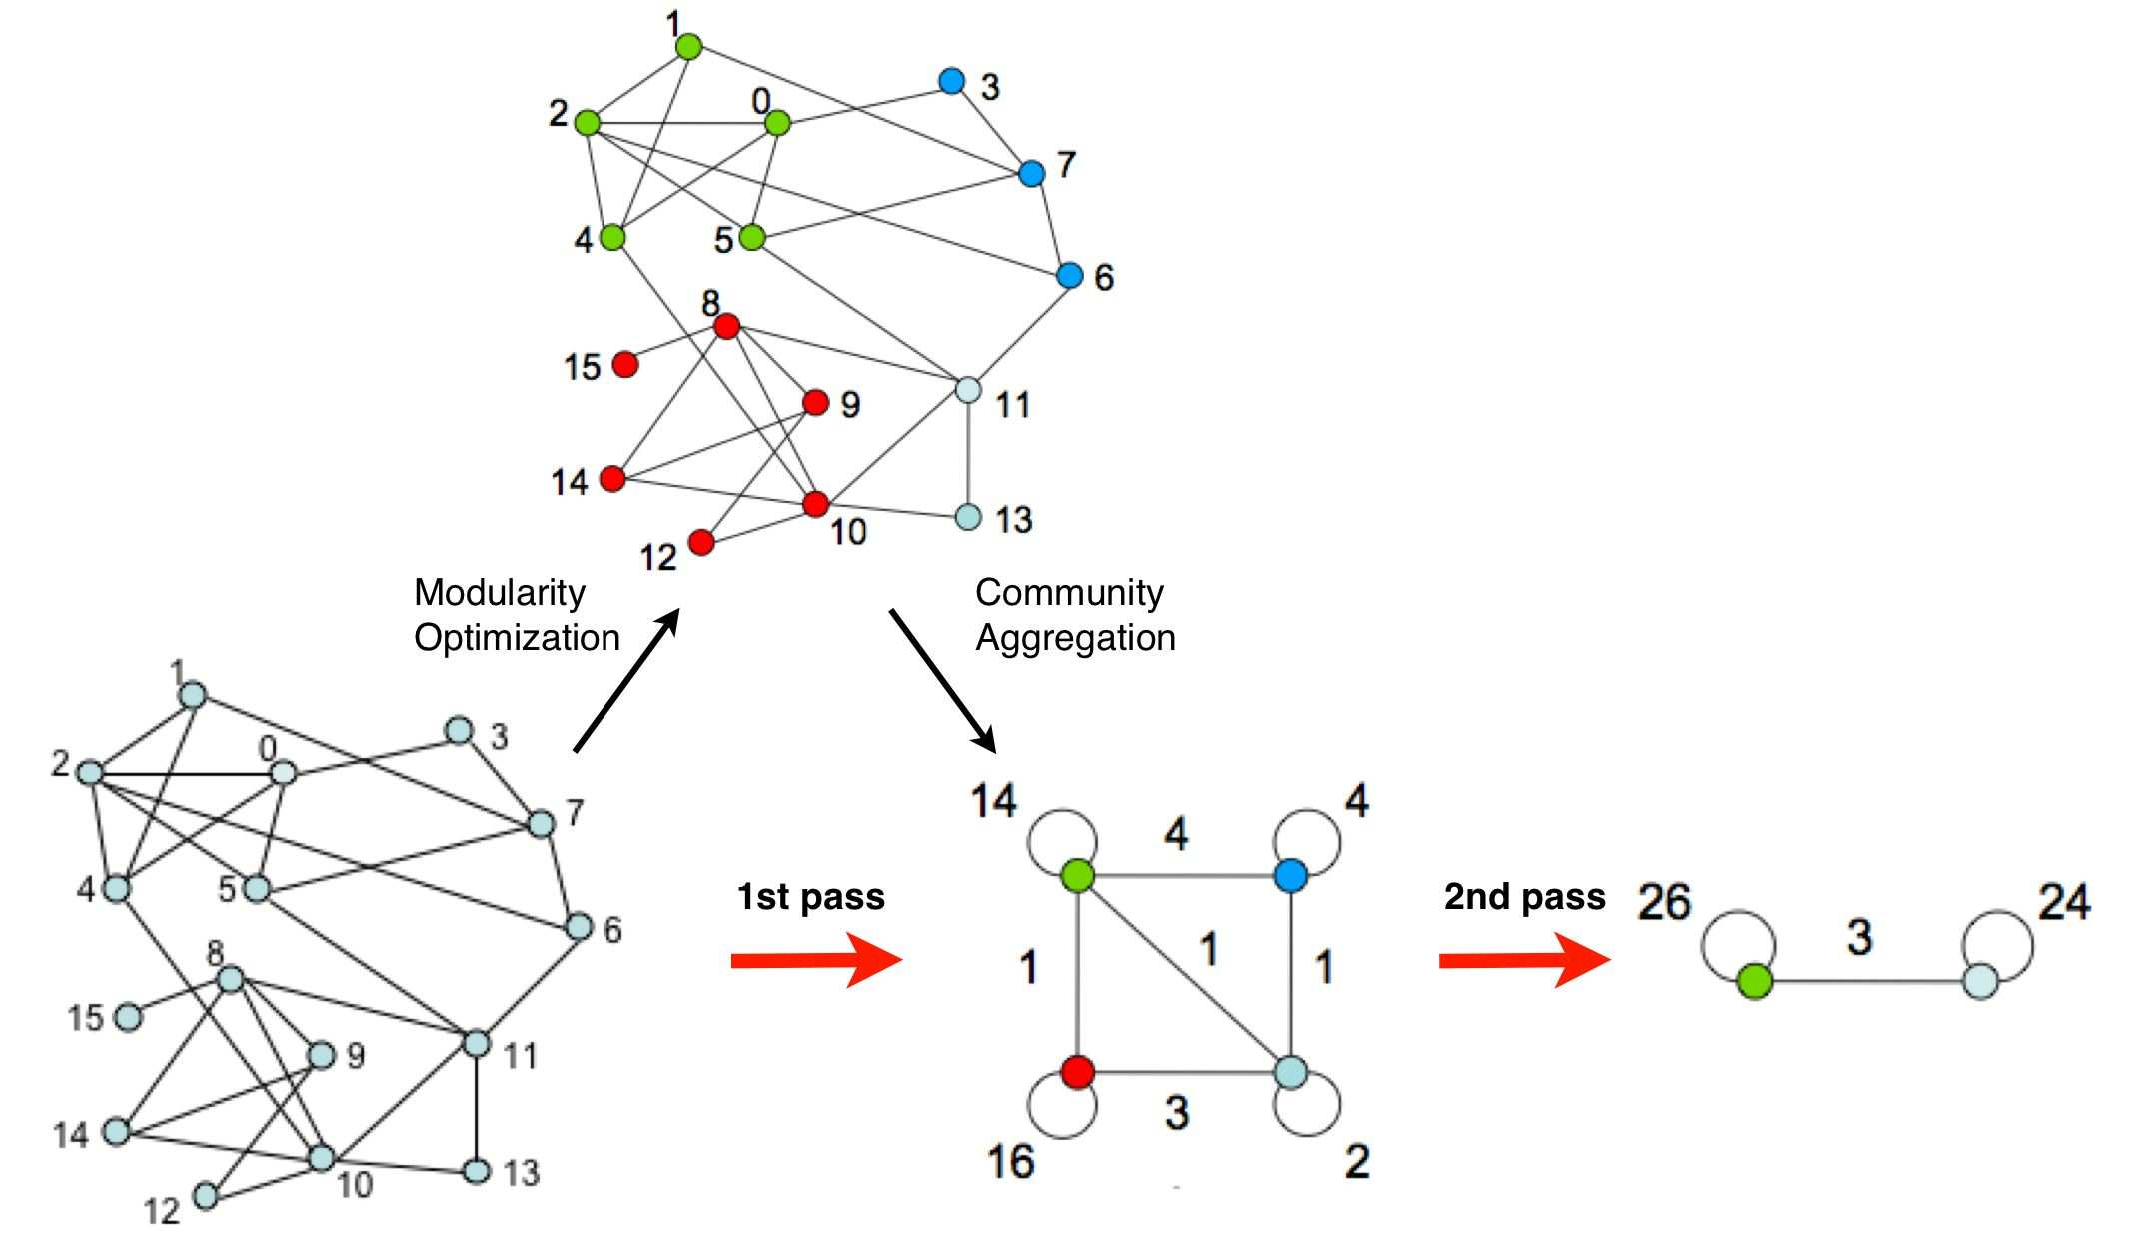
\includegraphics[width=1\linewidth]{0-resources/blondel_scheme}
	\caption{Scheme of the Louvain algorithm. This image is reprinted from \cite{Blondel_2008}.}
	\label{fig:blondelscheme}
\end{figure}
This greedy algorithm its quite simple. There are two phases that are repeated iteratively: the optimization phase and the aggregation phase. At the start of the optimization, each nodes is assigned to its self-community, i.e. each node belongs to a community composed by only itself. 
In the first phase, for each node $i$, we evaluate for each community $j$ that have at least one node in the neighbour of $i$ $N(i)$, the gain of modularity $\Delta Q_{i \rightarrow c_j}$ that we have if we remove $i$ from its community $c_i$ and we assign it to $C_j$.
To due this, we can use the equations (\ref{ModularityC}) to calculate the modularity in current configuration $Q_{i\rightarrow c_i}$ and the modularity $Q_{i\rightarrow c_j}$ in the configuration where $i$ is assigned to $c_j$ and subtract, but this is quite inefficient. Instead, we can calculate directly  $\Delta Q_{i \rightarrow c_j}$:
\begin{equation}
\Delta Q_{i \rightarrow c_j} = \frac{l_{i\rightarrow c_j} - l_{i\rightarrow c_i / \{i\}}}{2|V|} + k_i \frac{k_{c_i / \{i\}} - k_{c_j}}{4|V|^2}
\end{equation}
where $l_{i\rightarrow c_j}$ is the sum of edges that connect $i$ to the community $c_j$, $k_i$ is the weight of the nodes $i$ and $k_{c_j}$ is the weight of the community $c_j$.
Then we define the subset $Z_i$ the set of community $c_z$ with $z \in N(i)$ such that:
\begin{align}
\Delta Q_{i \rightarrow c_z} \geq \Delta Q_{i \rightarrow c_j} && \forall j \in N(i)
\end{align}
If more there is more than one community in the group, one community $c_z^*$ was selected using a braking rule, otherwise we pick the only community in $Z_i$. If $\Delta Q_{i \rightarrow c_z^*} > 0$, we move the node $i$ to the community $c_z^*$. \\
This process is applied repeatedly and sequentially for all nodes while modularity score increases. When no more improvement can be reach, the second phase start. In this phase a new network was created from the results of the previous phase: in the new graph, the nodes are the communities found, and the edge between them are given by the sum of the links between nodes that belong to the corresponding communities (edge between nodes in the same communities lead to self-loop). Then we reapply the first step and then the second one until no more improvement is obtained. An example of the algorithm is shown in the Figure \ref{fig:blondelscheme}. \\
The complexity of this algorithm is $O(m)$ where $m$ is the number of the edges of the graph, due to the fact that we can compute the
gains in modularity for each neighbour easily. Respect to the previous approach, this techniques reaches the goal of the execution in linear times. Indeed, this algorithm can create an entire hierarchies of partitions and this can be useful to avoid the resolution limit problem: we can analyze in the dendrogram the intermediate solutions to observe its structure with the desired resolution \cite{Blondel_2008}.
\subsection{Pruning}
This algorithm even in the first formulation is quite efficient, but large network analysis requires improvement to be executed quickly. The parallel techniques are very useful for this task and it will be presented in the next chapter. Now we focus on a method that speed-up the computations in the sequential field but that is also suitable in parallel.\\
The first optimization phase is the most time consuming ones \cite{Blondel_2008}, consuming about 80\% of the time \cite{wickramaarachchi2014fast}. To reduce the impact of this first phase, in literature were proposed various approach. For example, in \cite{rand}, V. A. Traag proposed to randomize the choice of the community which you want to assign the nodes between the communities of the neighbour. The idea behind these techniques is that the nodes tend to be in a "good". This technique performs well sequentially if the graph were the community structure is well defined. Instead, in parallel behaviour, this method doesn't be so good due to the fact, each node changes communities simultaneously, and there is no way to prevent simultaneous swaps without introducing some overhead and this may lead to a convergence problem. For this reason, we choose another technique more parallel friendly, introduced by Ozaki et. al \cite{pruning}. Now we present this simple and efficient technique of optimization for this algorithm that doesn't afflict the quality of the partitions. This method makes a pruning of the nodes in the optimization phase in order to compute the maximum delta modularity for only the nodes that have the potential to change community.
Every time a node $i$ changes community from $X$ to $Y$, its affect the $\Delta Q$ of its neighbourhood and all nodes linked and in $X$ and $Y$. Referring to \ref{ModularityC}, we describe all these cases:
\begin{itemize}
	\item Nodes in $X$ that aren't connected to $i$:  for those nodes, the value of $\Delta Q_X$ increase because of the degree of the community $k_X$ decrease without affecting the value of $l_X$.
	\item Nodes in $Y$ that aren't connected to $i$: for those nodes, the value of $\Delta Q_Y$ decrease because the degree of the community $k_Y$ increase without affecting the value of $l_Y$.
	\item  Nodes that are linked to a node in $X$, but not to $i$: for those nodes, the value of $\Delta Q_X$ increase because of the degree of the community $k_X$ decrease without affecting the value of $l_X$.
	\item  Nodes that are linked to a node in $Y$, but not to $i$: for those nodes, the value of $\Delta Q_Y$ decrease because the degree of the community $k_Y$ increase without affecting the value of $l_Y$.
	\item Nodes that are linked to $i$ in $X$:
	in this case both $k_X$ and $l_X$ decrease for $\Delta Q_X$..
	\item Nodes that are linked to $i$ in $Y$:
	in this case both $k_Y$ and $l_Y$ increase for $\Delta Q_Y$.
	\item Nodes that are linked to $i$ but that are not either in $X$ or in $Y$:
	in that case afflict both $\Delta Q_X$ and $\Delta Q_Y$ (increase $k_X$, $l_X$, $k_Y$ and $l_Y$).
\end{itemize} 
The nodes considered in first and the fourth case, doesn't have the potential to change community: in the first case one increase the value of $\Delta Q_X$ that is the maximum (because they are already in the community $X$); in the fourth case one decrease the values of $\Delta Q_Y$ that aren't the maximum (because they are not in the community $Y$). In all other cases, there is a chance that some nodes change community. In the Figure \ref{fig:pruning}, the white nodes are the nodes that doesn't have the potential to change community, instead the black and striped ones are the ones that may have. Considering only this nodes, the computation time will be reduced without reducing the quality of the partition.
\begin{figure}
	\centering
	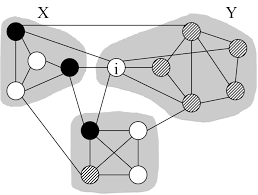
\includegraphics[width=0.7\linewidth]{0-resources/pruning}
	\caption{Example of graph where the nodes $i$ changed community from $X$ to $Y$. This image is reprinted from \cite{pruning}.}
	\label{fig:pruning}
\end{figure}\\
The optimization proposed by Ozaki et. al consists to create a set of nodes during the iteration of the optimization that will be analyzed in the next step: at the start of the optimization phase, an empty set $S$ is created and every time a node $i$ change its community, each nodes in its neighbourhood that doesn't belong to the new community is add to $S$. The next iteration consider only the nodes in $S$ and the process is iterated. They consider only one of the four previous categories of nodes: this is because calculating all nodes (explicitly the ones in the second and third group) introduce overhead and this group is the most influential for $\Delta Q$ \cite{pruning}. The selected nodes to be add to $S$ are the black one in the Figure \ref{fig:pruning}. 
The experimental result show that reduce the computational time by up to 90\% compared with the standard Louvain algorithm. In terms of accuracy, surprisingly, the modularity is almost the same,  not only the final one, but also the transition of the modularity during the iterations \cite{pruning}. 
\newpage
\subsection{Parallel Implementations}
Now we present various approach that was used in literature to improve the performance of the Louvain algorithm. We can divide the parallelization techniques in two different class: the coarse grained approach and the fine grained approach. The methods in the first class divides the nodes in some sets and the modularity are processed sequentially independently for each set. When all sets are analyzed, the algorithm merge the results for the next phase. Instead, the second approach consider each nodes independently. The best modularity were calculated for each node simultaneously, therefore the decision of the new community for each node is based on the previous configuration. Wickramaarachchi et al. \cite{wickramaarachchi2014fast} proposed one of the first coarse algorithm: in the first iteration, the algorithm partition the graph in subgraphs and the execution were performed simultaneously and independently on each partition. Edges that cross the partition were ignored. In terms of quality, they showed that ignoring edges cross partition edges does not impact to the quality
of the final result. \\
In 2015, both Staudt and Meyerhenke \cite{staudt2015engineering} and Lu et al. \cite{lu2015parallel} proposed an fine grained implementation based on OpenMP. To compute $Q_{i \rightarrow c_j}$ for each nodes $i$ and each communities $c_j$ in neighbourhood of $i$ , the algorithm  must calculate $l_{i\rightarrow c_j}$(i.e. the sum of edges that connect $i$ to the community $c_j$ ). These values may change in every new configuration: for this reason we must have a method to get it them fast. In \cite{staudt2015engineering}, they try to associate each node with a map in which the edge weight to neighbouring communities was stored and updated when node moves occurred, but they discover that introduced too much overhead.
Instead, recalculating each time the weight to neighbour communities each time a node is evaluated turned out to be faster. Therefore, they proposed to use a \verb|map| for each node as accumulator of his edges to calculate every $l_{i\rightarrow c_j}$. Instead the total weights of each community $k_{c_j}$ is stored and updated every time a nodes change community. The same scheme is used in \cite{lu2015parallel}. A more complex schema was proposed by Que et al. \cite{que2015scalable}: they proposed an algorithm based on a communication pattern that permit to propagate the community state of each nodes. 
Due to his complex behaviour, this schema is hard to implement on the GPU.\\
Forster in \cite{forster2016louvain} presented a GPU implementation based on the first two previous OpenMP version: he reports a speed-up to a factor of 12, but in the paper there isn't information about the quality of the partition. Following, the algorithm preposed form Naim et al. \cite{naim2017community} parallelize the hashing of the edges both in optimization and also in the aggregation phase. In addition, they partitioning the vertices into subsets on their degrees in order to obtain an even load balance between threads.
A different implementation was proposed by Cheong et al. \cite{cheong2013hierarchical}: it is a multi-GPUs implementation that used a coarse grain model between the GPUs and than a fine grain model for the computation of the modularity of each sub-graphs. This algorithm its also peculiar because doesn't use hashing to calculate the modularity but sort each neighbour list
based on the community ID of each neighbouring vertex.

	\newpage
	\section{PSR-Louvain and PH-Louvain}\label{GPUalg}
In this chapter, we present two novel parallel implementations of the Louvain algorithm: both versions implement the pruning presented by Ozaki et. al. \cite{pruning}.  The two algorithm differ on the way in which they accumulate the edges to calculate $l_{i\rightarrow C_j}$  (see formula \ref{ModularityC}). The first one, the PSR-Louvain, where PSR stands for Prune, Sort and Reduce Louvain, is based on the sort-reduce pattern: it sorts the list and performs a reduction of consecutive values with the same key. We also use a reduction on a sorted array to compute the maximum values of modularity for each node. 
The second algorithm, PH-Louvain, where PH stands for Prune and Hashmap Louvain, uses a map to accumulate that values.
In this chapter, we present firstly the the algorithms, then a special speed-up technique of the first iteration of the optimization phase included in both algorithms and finally the data structure and the implementations details.

\subsection{PSR-Louvain}\label{Prune-Sort-Reduce}
The Prune, Sort and Reduce Louvain algorithm is the first version of the algorithm that we present in this thesis. As the sequential Louvain algorithm, we can divide it into two steps iterated alternately: the optimization phase and the aggregation phase. 
Furthermore, we divide the optimization phase in eight sub-phases, in which the operations are executed in parallel.
This algorithm takes in input a graph stored as a list of edges, where each entry is a tuple $(i,j,w)$: $i$ is the source node, $j$ is the destination node and $w$ is the weight of the edge; in this algorithm, even if the graph is undirected, we consider every edge twice reverting the order of the source and the destination. This list is sorted by $(i,j)$. In the beginning, we have each node is assigned to a community composed only by itself.
The weight of each node, a map that associate at each nodes the corresponding communities and the total weight of each communities. At the first iteration each node is in a community by itself and the total weight of each community corresponding at the weight of the unique node in it. The sub-phases of the optimization phase are the following:\\
\begin{figure}[t]
	\centering
	
\includegraphics[width=1\linewidth]{0-resources/PSR-Louvain-Schema}
	\caption{Schema of the PSR-Louvain algorithm.}
	\label{fig:psr-louvain-schema}
\end{figure}

\begin{enumerate}
	\item \textbf{Copy sub-phase:}  this algorithm implements firstly the pruning presented by Ozaki in the parallel behaviour \cite{pruning}. Therefore, in the first step, we copy from the list of edges, all those that belongs to a node that we have consider in this iteration. To due this, we check on a support vector if the source nodes of the edges have a neighbour that has change community according to the criteria presented in Chapter \ref{prun}. We use a support vector to check if the node matched the requirement: in position $i$ there is a True if the nodes $i$ matched the criteria in the previous iteration, False otherwise. At the first iteration all the nodes are considered. We exclude from the copy also the self-loops because we don't consider them in the computation of the various values of $\Delta Q$. Besides, in this phase, we don't copy destination nodes $j$ but we substitute that values with the associated community $c_j$. Therefore, we obtain a list of tuples that contain the source node $i$, the community $c_j$ related to the linked node $j$ and the weight of the edge $w$.  
	
	\item \textbf{Sort sub-phase:} This algorithm uses a scheme of computation inspired by \cite{cheong2013hierarchical}. In the second phase, we sort the data obtained in the first phase. Given the list of tuples $(i, c_j, w)$ created in the previous sub-phase, we sort it using the pair $(i, c_j)$ as key.  At the end of this phase, we have that all the tuples $(i, c_j, w)$ with the same $(i, c_j)$ are consecutive. Besides, all the tuples with the same source node $i$ are consecutive.
	
	\item \textbf{Reduce sub-phase:} in this step we perform a reduction by key, i.e. we sum up all consecutive values with the same key. We use as key the tuple $(i, c_j)$: doing this, we obtain a unique tuple $(i, c_j,$  $l_{i\rightarrow c_j})$ for each pair $(i, c_j)$ where $l_{i\rightarrow c_j}$ is the sum of all the weights of edges that links the node $i$ with a node in the community $c_j$. We need this value to calculate later the $\Delta Q_{i\rightarrow c_j}$.
	
	\item \textbf{Self community counting  sub-phase:} In this phase, we isolate all the tuples  $(i, c_j, l_{i\rightarrow c_j})$ such that 
	$c_j$ is the actual community for the nodes $i$, i.e. $c_i$. We need to isolate these values $l_{i\rightarrow c_i}$ because we use it in the next phase to compute the various values of $\Delta Q$ (Eq. (\ref{delta_q})).
	
	\item \textbf{Compute Delta sub-phase:} Now we can calculate the $\Delta Q_{i\rightarrow c_j}$ for each tuple using the Eq. (\ref{delta_q}) , because we calculated all the $l_{i\rightarrow c_j}$ in the previous steps and we have the weights of the communities and the weights of the nodes in input. After the computation, we obtain a list of tuple $(i, c_j, \Delta Q_{i\rightarrow c})$.
	
	\item \textbf{Select Max sub-phase:} Now we need to isolate the maximum $\Delta Q_{n\rightarrow c_j}$ for each node $n$. Considering that the vector is already sorted, we can perform this operation using another reduction but, in this case, we return only the maximum weight. We execute this operation using the nodes $i$ as keys.  After this step, we have exactly one tuple  $(i, c_z, \Delta Q_{i\rightarrow c_z})$  for each nodes $i$ where $c_z$ is the community that gives the maximum increase in modularity $\Delta Q_{i\rightarrow c_z}$ if the node $i$ is assigned to $j$.
	
	\item \textbf{Update Community sub-phase:}\label{update_com} In this step, we update the community for each node if the value of $\Delta Q_{i\rightarrow c_z}$ is greater than 0. We also update the related community weights: we remove the weight of the node from the previous community and we add it to the new one. These operations are implemented as atomic to avoid concurrent operations.  We also keep track if each node changed or not its community. We remark that this
	vector is different respect to the array that we use in the first step. In the following step, we create the pruning vector from this one.

	
	\item \textbf{Update Pruning sub-phase:}\label{update_prun} : To update the vector that handles the pruning
	criteria, we firstly set all its elements to zero. After that, a method takes each
	edge of the graph and check if the destination edge has changed its communities
	in the previous iteration: if this happened, the corresponding node value is set
	to True. This update operation is not atomic, because multiple threads can
	set only a True to the same position and there aren’t conflict.

\end{enumerate}
Afterwards, we compute the new modularity score and than we compare the obtained value with the old one: if the value is larger than a given threshold, we repeat these steps, otherwise we start the aggregation phase. We highlight that we can not add directly the various $\Delta Q$ obtained in the optimization step to the old modularity
like the sequential algorithm, because all nodes change communities simultaneously and consequently this value is not reliable any more.
The Algorithm \ref{alg:sort-optimization} summarize the phase.
\begin{algorithm}
	\caption{Prune-Sort-Reduce: Optimization phase}\label{alg:sort-optimization}
\begin{algorithmic}
\Procedure{optimizationPhase}{Graph $G$, Community $C$}
	\State $pruning = vector(True, n\_nodes)$
	\State $old\_delta = 0$
	\State $delta = modularity(G,C)$
	\While{ $delta - old\_delta <$ THRESHOLD}
		\State $node\_to\_community = \text{[ ]}$
		\State $self\_values = \text{[ ]}$
		\State $ $
		\Comment{copy}
		\For{\textbf{each} edge $(i,j,w)$ in $G$ \textbf{in parallel}}
			\If{$pruning[i]$ == $True$ and $i$ != $j$}
				\State $node\_community.append(i,C[j],w)$
			\EndIf
		\EndFor 
		\State $ $
		\Comment{sort}
		\State $node\_community.parallel\_sort(by= \text{source, community})$
		\State $ $
		\Comment{reduce}
		\State $node\_community.parallel\_reduce(\text{ }by= \text{source, community}, $
		\Statex[12] $operation= \text{sum})$
		\State $ $
		\Comment{self-counting}
		\For{\textbf{each} $(i,cj,l)$ in $node\_community$ \textbf{in parallel}}
		\If{$C(i)$ == $cj$}
			\State $self\_values[i] = l$
		\EndIf
		\EndFor
		\State $ $
		\Comment{delta}
		\State $s = size(node\_community)$
		\For{$z$ in $[0,1,...,s]$ \textbf{in parallel}}
			\State $node\_community[z] = compute\_delta(node\_community[z],$ 
			\Statex[14] $self\_values,$ 
			\Statex[14] $communities\_weight,$
			\Statex[14] $nodes\_weight)$
		\EndFor
		\State $ $
		\Comment{max}
		\State $node\_community.parallel\_reduce(\text{ }by= \text{source},$
		\Statex[9] $operation= \text{max})$
		\State $ $
		\Comment{update community}
		\State $is\_change = vector(False, n_nodes)$
		\For{\textbf{each} $(i, cz, delta)$ in node\_to\_community \textbf{in parallel}}
			\If{$delta > 0$}
				\State $atomicAdd(communites\_weight[C[i]], -nodes\_weight[i])$
				\State $atomicAdd(communites\_weight[cz], nodes\_weight[i])$
				\State $C[i] = cz$
				\State $is\_change[i] = True$
			\EndIf
		\EndFor
		\State $ $
		\Comment{update pruning}
		\For{\textbf{each} edge $(i,j,w)$ in $G$ \textbf{in parallel}}
			\If{$is\_change[j]$ == $True$}
				\State $pruning[i] = True$
			\EndIf
		\EndFor
		\State $old\_delta = delta$
		\State $delta = modularity(G,C)$
	\EndWhile
	\EndProcedure
	\end{algorithmic}
\end{algorithm}\newpage
\noindent The aggregation phase uses several similar concepts presented previously, and we can divide it into four sub-phases in which the operations are executed in parallel:
\begin{enumerate}
	\item \textbf{Re-indexing communities sub-phase:}\label{Re-indexing} in the first phase, before the graph contraction, we assign a new id to the communities. Actually, we have only certain communities associated to the nodes respect to the initial configuration: for example, if a nodes $i$ change community from $c_1$ to $c_2$ in the first iteration of the optimization phase, no nodes are assigned to $c_1$ after the update and no nodes can select the communities $c_1$ from that moment. This cause a useless waste of memory if we continue to keep all those unused values in the community weight. For this reason, we need to create a map to rearrange the communities index.
	First, we create a support vector such that at the position $c$ there is a 1 if the community $c$ has a weight greater than 0 (i.e. there is at least one node assigned to this community). Then we perform a prefix sum on this vector: in this way at the position $c$ there is the new index incremented by one for the community $c$ (please note: incremented by one because we counting from zero).
	 We remark that even if the empty communities are still mapped with this method and have the same indexes of the community at the preceding position respect them, we doesn't have any conflict because we doesn't use these entry.
	 When this renumbering map is ready, we start the next phase.
	\item \textbf{Transform edges sub-phase:} In this step, all the pairs of edges $(i, j)$ of the original graph are transformed in the pair $(c_i, c_j)$ where $c_i$ ($c_j$) is the community associated to $i$ ($j$). In this phase, we also apply the map to renumber the communities that we create in the previous step. 
	\item \textbf{Sort-Reduce sub-phase:} In this phase we sort all the edges $(c_i, c_j, w)$ using as a key for the sorting the pair $(c_i, c_j)$. After this, we reduce the edges vector still using as a key $(c_i, c_j)$. After this step we have contract the graph summing up all the edges that lay between two communities.
	\item \textbf{Update variables sub-phase:}\label{updategraph}  In the last step, we update all the support value in the graph object, like the number of the nodes, the number of edges, the nodes weights. We also reset the communities object reordering the communities weight according to the re-indexing map and assigning each node to a community composed only by itself.
\end{enumerate}
The Algorithm \ref{alg:sort-aggregation} summarizes this phase. 
The PSR-Louvain continues to alternate this two phases until we can not have further improvement in the modularity update. In this version of the algorithm, we keep only the best result to not occupy several device memory, but it is possible trivially save the intermediate result adding a step that save the clustering results after the re-indexing sub-phase (in this way we have consistent indexing among the dendrogram).
\begin{algorithm}
	\caption{Prune-Sort-Reduce: Aggregation phase}\label{alg:sort-aggregation}
	\begin{algorithmic}
		\Procedure{aggregationPhase}{Graph $G$, Community $C$}
		\State $ $
		\Comment{re-indexing}
		\For{$i$ in size($communities\_weight$) \textbf{in parallel}}
		\If{ $communities\_weight[i]$  == $0$)}
		\State $map[i] = 0$
		\Else
		\State $map[i] = 1$
		\EndIf
		\EndFor 
		\State $map.prefix\_sum()$
		\State $ $
		\Comment{transform}
			\For{\textbf{each} edge $(i,j,w)$ in $G$ \textbf{in parallel}}
			\State $\text{Substitute } i , j \text{ with } map[C[i]], map[C[j]]$
		\EndFor 
		\State $ $
		\Comment{sort-reduce}
		\State $G.edges.parallel\_sort(by= \text{"source, community"})$
		\State $G.edges.parallel\_reduce(by= \text{"source, community"}, $
		\Statex[9] $operation= \text{"sum"})$

		\State $ $
		\Comment{update}
		\State $G.update()$
		\State $C.update(G)$	
		\EndProcedure
	\end{algorithmic}
\end{algorithm}
\newpage
\subsection{PH-Louvain}
The second version of the parallel Louvain algorithm is quite similar to the previous pruning approach, but uses a different way to aggregate the weights of edges that link a node to the same community: we use a special global hashmap instead of sorted vector.
Using a map to accumulate some values by its key is a standard approach to solve this problem because the map allows to retrieve and insert an object in $O(1)$ time. 
To obtain this performance, the hashmap uses a function named hash function to dispose at random the objects in the memory. This creates a problem on the GPU because uncoalesced memory accesses is an order of magnitude slower than sequential memory accesses. 
To overcome this problem this map uses a system of open-addressing based on the cuckoo hashing: this type of map is the one that performs better on the GPUs \cite{alcantara2012building}, thanks to a simple and efficient management of the conflicts. This map uses 64 bits for the key and 32 bits for the value. We choose to use 64 bits for the key because we need to store a pair of 32 bits keys (the pair $(node, community)$ in the optimization phase and the $(community, community)$ pair in the aggregation phase). This map has $r$ different hash function, each one associated to an id $r_i$ where $i \in [0, r-1]$. When we insert a new pair key-value $(k,v)$, we use the hash function with id $r_0$ to compute the position of the new key $v$: if the slot is empty, we add the key and the value, we use the next function $r_1$ otherwise. We continue to search a empty slot following this schema: if $r_i$ is not empty, we retry to insert the pair with function $r_{i+1}$. If all the function fails to insert the new pair, we raise an error.\\ 
The main difference between this map and the classic cuckoo hashing is that 
the original version of the map when we try to insert an entry in a position that is already filled, the map remove the old pair key-value, insert the new one and try to find a new position for the old value using another hash function.  
In our map, we don't "kick out" the old key when we have a conflict in order to find a new memory address for it, but we hash with a different function the pair that we have to insert: this because to make a classic cuckoo hashing, we need a set of atomic operations for 128bits to do the "kick out" operation in parallel without generating race condition. This type of atomic operation in CUDA can be done only on variable up to 64 bits. Besides, this map has another special feature: if we insert a pair $(k,v)$ and there is already an entry in the table with a key $k$, the map automatically sum the values $v$ to the one stored in the map. Indeed, we use this map only to aggregate values, and for this reason, we design it to this operation as fast as possible. The last feature that we add to this table is the contract table operation: this methods the map in pair of contiguous vector re-arranging the memory, in order to allow us to access to each pair key-value sequentially. After this operation, we can not get the entry using the hash function, because the memory is re-organized. We use this operation before the computation of $\Delta Q$ to increase the performance and still working considering the edges $(nodes, communities)$ independently. 
\begin{figure}[t!]
	\centering
	
\includegraphics[width=1\linewidth]{0-resources/PH-Louvain}
	\caption{Schema of the PH-Louvain algorithm}
	\label{fig:ph-louvain}
\end{figure}
Now we present the algorithm. At the start of the optimization phase we have each edge represented as a tuple $(i,j,w)$,  a the weight of each node,  a map that associates each nodes with the corresponding communities  and the the total weight of each communities like the previous algorithm. 
We divide the optimization phase into six sub-phases:
\begin{enumerate}
	\item \textbf{Fill Map sub-phase:} in the first step, for each edge $(i,j,w)$, we insert into the map the tuple $(n, c_j, w)$ where $c_j$ is the community associated to the destination nodes $j$. We use as a key the pair $(n,c_j)$.
	We consider only the tuple that has the source node that matching the criteria presented in Chapter \ref{prun}. We use a support vector identical to the one presented in the previous algorithm. We also exclude all the self-loops in this phase. At the end of this step we obtain a map where every non-empty entry has the form $(i, c_i, l_{i \rightarrow c_j})$. The map also isolate in a different vector each values $l_{i \rightarrow c_i}$ such that $c_i$ is the community of the nodes $i$ is stored at position $i$. This operation was made because in the delta step, after the contraction, we can not get any more the position of the entry using the hash function, and we need a method to get the nodes communities weights quickly. 
	
	\item \textbf{Contract Table sub-phase:} in the first step, using a map to calculate $l_{i \rightarrow c_j}$ allows accessing to the memory address in $O(1)$ time for each edge. But to compute the relative delta and the maximum, we have to access the memory using an uncoalesced memory access pattern. In addition, we have no idea of how and which community are in the neighbourhood of a given node: many application allocates a thread for each edge, transform the edge destination from nodes to community and then check the maximum. This approach lay to check multiple time the score of the community $c$ if two neighbours of the nodes $n$ are in $c$. To overcome this problem, we contract the table: the vector that composed the table are re-organized in order to permit sequential access, without empty slots between the entries. After this operation, the map becomes a vector containing the tuples $(i, c_j,l_{i \rightarrow c_j})$. The support vector with the sum of edges of the node that connects it with another in the same community is not re-arranged by this operation.
	
	\item \textbf{Compute Delta sub-phase:} now we can compute the $\Delta Q_{i\rightarrow c_j}$ for each tuple $(i, c_j, l_{i \rightarrow c_j})$ using the Eq. (\ref{delta_q}). The result overwrites the last value in the tuple (we doesn't need that value any more). To get the sum of edges that connect the nodes to its actual community, we use the vector created in the first step.
	
	\item \textbf{Select Max sub-phase:} now we have a vector of tuple $(i, c_j, \Delta Q_{i\rightarrow c_j})$. Now we have to select the pair $(c_i, \Delta Q_{i\rightarrow c_j})$ for each node $i$ such that $\Delta Q_{i\rightarrow c_j}$ is maximum. We can not use as the previous algorithm a reduce operation because we haven't a sorted array and the sorting operation is too expansive. Instead, for each tuple, we check if the value $\Delta Q_{i\rightarrow c_j}$ is greater compered to the one of the tuple saved in a support array at the position $i$: if it is, we substitute the old value with the new one, we do nothing otherwise. To avoid race condition in the insert, these operation are executed atomically. At the end of this step, we have exactly one tuple $(i, c_z, \Delta Q_{n\rightarrow c_x)}$ for each node $i$, like the previous algorithm.
	
	
	\item \textbf{Update Community sub-phase:} This phase update the community just like the one presented in the Prune-Sort-Reduce version (\ref{Prune-Sort-Reduce}, optimization sub-phase \ref{update_com}).
	
	\item \textbf{Update Pruning sub-phase:} This phase create the array with the pruning information just like the one presented in the Prune-Sort-Reduce version (\ref{Prune-Sort-Reduce}, optimization sub-phase \ref{update_prun}).
\end{enumerate}
The Algorithm \ref{alg:hash-optimization} summarizes this phase.
\begin{algorithm}
	\caption{Hashmap: Optimization phase}\label{alg:hash-optimization}
	\begin{algorithmic}
		\Procedure{optimizationPhase}{Graph $G$, Community $C$}
		\State $pruning = vector(True, n\_nodes)$
		\State $old\_delta = 0$
		\State $delta = modularity(G,C)$
		\State $ $
		\While{ $delta - old\_delta <$ THRESHOLD}
		\State $ $
		\Comment{fill map}
		\For{\textbf{each} edge $(i,j,w)$ in $G$ \textbf{in parallel}}
		\If{$pruning[i]$ == $True$ and $i$ != $j$}
		\State $hashmap.insert(i,C[j],w)$
		\EndIf
		\EndFor 
		\Comment{contract}
		\State $list = hashmap.contract()$
		\State $ $
		\Comment{delta}
		\For{$z$ in size(list) \textbf{in parallel}}
		\State $list[z] = compute\_delta(list[z], hashmap.self\_values,$ 
		\Statex[10] $communities\_weight, nodes\_weight)$
		\EndFor
		\State $ $
		\Comment{max}
		\State $result = \text{[ ]}$
		\For{\textbf{each} $(i, cj, delta)$ in list \textbf{in parallel}}
		\State $\text{START OF THE ATOMIC BLOCK} $
		\State $(i, cj_{old}, delta_{old}) = result[z]$
		\If{$delta > delta_{old}$}
		\State $result[z] = (i, cj, delta)$ 
		\EndIf
		\State $\text{END OF THE ATOMIC BLOCK} $
		\EndFor
		\State $list = result$
		\State $ $
		\Comment{update community}
		\State $is\_change = vector(False, n_nodes)$
		\For{\textbf{each} $(i, cz, delta)$ in list \textbf{in parallel}}
		\If{$delta > 0$}
		\State $atomicAdd(communites\_weight[C[i]], -nodes\_weight[i])$
		\State $atomicAdd(communites\_weight[cz], nodes\_weight[i])$
		\State $C[i] = cz$
		\State $is\_change[i] = True$
		\EndIf
		\EndFor
		\State $ $
		\Comment{update pruning}
		\For{\textbf{each} edge $(i,j,w)$ in $G$ \textbf{in parallel}}
		\If{$is\_change[j]$ == $True$}
		\State $pruning[i] = True$
		\EndIf
		\EndFor
		\State $ $
		\State $old\_delta = delta$
		\State $delta = modularity(G,C)$
		\EndWhile
		\EndProcedure
	\end{algorithmic}
\end{algorithm}
\newpage
\noindent
We continue to execute this step until the difference in modularity between the configuration drops below a given threshold. The consideration of the computing of $\Delta Q$ in parallel behaviour presented in the previous chapter is still valid. 
The aggregation phase of this algorithm use once again the map to aggregate, but the key in this context is composed of $(community_source, community_destination)$. We can divide this phase in four sub-phase like the previous version:
\begin{enumerate}
	\item \textbf{Re-indexing communities sub-phase:} In this sub-phase we associate each community to a new id to reduce the waste of memory. This sub-phase is identical to the sub-phase with the same name presented in the PSR-Louvain description (\ref{Prune-Sort-Reduce}, aggregation sub-phase \ref{Re-indexing}). 
	\item \textbf{Communities map sub-phase:} In this step, all the tuple of edges $(i, j, w)$ of the original graph are inserted in a hash table. Before the insertion, we transform each entry in the tuple $(r_i, r_j, w)$ where $r_i$ is an index of the community associated with $i$ after the remapping. We use as key the pair $(r_i, r_j)$. At the end of this step, we have each edge of the new graph, because we sum up all the edges that lay between two communities.
	\item \textbf{Contract-sort sub-phase:} At the beginning of this phase, we have a map containing all the edges of the new graph. However, the graph object store the edges information using three ordered vectors, so we have to re-organize the information stored in the unordered and uncoalesced map. To do this, we use the contract operation to transform the map in a vector of tuple $(c_i, c_j, tot)$ and then we sort the arrays according to the order of the first one. Finally, we have the updated graph.
	\item \textbf{Update variables sub-phase:} This phase update the new graph and the related communities object just like the one presented in the Prune-Sort-Reduce version (\ref{Prune-Sort-Reduce}, aggregation sub-phase \ref{updategraph}).
\end{enumerate}
The Algorithm \ref{alg:hash-aggregation} summarize this phase. 
Like the previous algorithm, this one continues to alternate the two main phases until no further improvement in the modularity update can be obtained.
\begin{algorithm}
	\caption{Hashmap: Aggregation phase}\label{alg:hash-aggregation}
	\begin{algorithmic}
		\Procedure{aggregationPhase}{Graph $G$, Community $C$}
		\State $ $
		\Comment{re-indexing}
		\For{$i$ in size($communities\_weight$) \textbf{in parallel}}
		\If{ $communities\_weight[i]$  == $0$)}
		\State $map[i] = 0$
		\Else
		\State $map[i] = 1$
		\EndIf
		\EndFor 
		\State $map.prefix\_sum()$
		\State $ $
		
		\Comment{map}
		\For{\textbf{each} edge $(i,j,w)$ in $G$ \textbf{in parallel}}
			\State $hashmap.insert(map[C[i]],map[C[j]],w)$
		\EndFor 
		
		\State $ $
		\Comment{contract-sort}
		\State $G.edges = hashmap.contract()$
		\State $G.edges.parallel\_sort(by= \text{"source, community"})$
		\State 
		
		\State $ $
		\Comment{update}
		\State $G.update()$
		\State $C.update(G)$
		
		\EndProcedure
	\end{algorithmic}
\end{algorithm}

\subsection{Speed-up the First Iteration in the Optimization Phase}\label{f-1}
In this chapter, we present an optimization technique that we add into our code to speed-up the first iteration of each optimization phase. We include this method in both versions of the algorithm presented previously. We focus this presentation on the Prune-Sort-Reduce version, even if the concept that allows us to optimize the algorithm is still present in the Hashmap version. At the beginning and also after each aggregation phase, we notice that we have a configuration in which each node is assigned to each self-community, i.e., each node $i$ is assigned to the community $c_i$ and it is the only node assigned to it. In this configuration, when in the copy sub-phase we transform each edge $(i,j)$ in the pair $(i,c_j)$ where $c_j$ is the community of the node $j$, we obtain the same original pair, because the index of $c_j$ is equal to $j$. In addition, considering that each node is assigned to a different community, we don't need the sort and reduce sub-phases, because the pairs $(i, j)$ are already sorted by the construction of the graph object ()we need a sorted vector for the select max sub-phase) and the reduction is useless, because all the pairs have a different composite key $(i, j)$.
Also the self-counting sub-phase is useless, because no edge that isn't a self-loop lay a node in the same community and during the copy sub-phase we excluding the self-loop from the computation. 
Considering all these facts, we choose to remove in the first iteration this three sub-phases and also to avoid the useless transformation in the copy sub-phase. For the Hashmap version of the algorithm, we still use this optimization based on the other version because we use the hashmap to aggregate different edges and this aggregation is no longer necessary.

\subsection{Data structure and implementation details}\label{impl-details}
The two main structures that we need to represent are the original graph and the community structure. Commonly a graph $G(V, E)$ is represented using its adjacency matrix: each node is associated with an incremental id in the range $(0, n-1)$ where $n$ is the number of nodes. To retrieve the weights of an edge between two nodes, we look to the values stored at the position $(id_1, id_2)$. As we say in the chapter \ref{3.1}, the community detection techniques are effective if executed on sparse graphs.  Therefore, if we use a matrix to represent a sparse graph, this matrix will have a lot of zeros. Even if this pattern allows to retrieve the weight of an edge in constant time, this data structure isn't suitable for a problem that involves millions of data because we need too much memory to allocate this matrix and it has several unused values. Therefore, we have the necessity of compress the adjacency matrix. To do this, we choose to represent it using a coordinate list (often referred to as COO). We have three vectors \verb|edges_source|,  \verb|edges_destination| and  \verb|weights| that contain respectively the ids of the rows, the ids of the columns and the values. The standard modularity optimization is computed on undirected graphs: this means that the adjacency matrix is symmetric and we can store in the COO list only the upper triangle of the matrix and we still have all the edges represented. Despite this observation, we store all the values of the adjacency matrix because we need those repeated values in these algorithms when we transform the destination node in the destination community. These vectors are also sorted by the pair $(source, destination)$ and there is a vector named  \verb|neighboorhood_sum| of length $n$ in which at position $i$ there is the starting position of the edges that have source $i$ in \verb|edge_source|. Thanks to this vector, we can retrieve fast all the neighbour of a given node. These particular COO lists are also known as compressed neighbour lists. In the graph object, we also store a vector named \verb| tot_weight_per_nodes| that associate each node $i$ to its degree, the total degree of the graph, the number of nodes and the number of the edges. We use \verb|thrust::device_vector| to store all this data on the GPUs memory. In summary, the graph object is the following:
\begin{lstlisting}[language=C++]
struct GraphDevice {
	unsigned int n_nodes;
	unsigned long n_links;
	double total_weight;

	thrust::device_vector<unsigned> tot_weight_per_nodes;
	thrust::device_vector<unsigned int> neighbourhood_sum;

	thrust::device_vector<unsigned int> edge_source;
	thrust::device_vector<unsigned int> edge_destination;
	thrust::device_vector<unsigned int> weights;
}
\end{lstlisting}
We design the community object so that it contains the graph associated with it. We notice that the maximum number of different communities is pair to the total number of nodes: this is also the configuration at the beginning of the algorithm. Considering this, we choose to identify each community with an incremental id in the range $(0, n-1)$, like we do previously with the nodes. Therefore, in the community object, we have a vector named \verb|communities| of length $n$ in which in the position $i$ there is the id of the community of the node $i$. Besides, there is a vector of size $n$ that associate each community to its total weight.  In summary,  the community object is the following:
\begin{lstlisting}[language=C++]
struct Community {
	GraphDevice graph;
	
	thrust::device_vector<unsigned int> communities;
	thrust::device_vector<double> communities_weight;
}
\end{lstlisting}
After the initial parsing, we use only the device memory to store the data. The GPU memory is related to the machine and is usually smaller than a RAM.
To reduce the memory used simultaneously during the optimization phase, the Prune-Sort-Reduce algorithm divides the edges in buckets of fixed size. 
The algorithm executes the sub-phases from the first to sixth on a bucket, stores the results and start the execution on another bucket. When all buckets are considered, we execute the last two updating sub-phases. This reduce the required memory used to store the data from $2*m$ (used to store two vector that can store all the nodes: one for the copy and one to store the reduced values) to $2*size(bucket) + n$ (two vector of the bucket size for the copy and the reduce operation and a vector to store the best result for each node). 
In order to compute the right maximum values of $\Delta Q$ for each node, we split the edges into buckets such that if there is an edge with source node n in the bucket, also all the other edges that belong to n are included. To perform this, we use the \verb|neighbourhood_sum| vector to select the right range. The Hashmap version implements a similar logic, performing repeatedly the the first four sub-phases on different buckets,  and then eventually update the communities and the pruning vector when all buckets are processed. We use buckets of maximum size equals to 50 000 000.\\
Both algorithms implements also the minimum label heuristic (Chapter \ref{parallel-imp}): we change communities only if the id of the new communities is lower than the old one for communities composed only by a single node to prevent the simultaneous swap. We also select the communities with the lowest id when we have multiple communities with the greatest $\Delta Q$ for the same node: this method leads to a faster convergence.

In the algorithms, each parallel sub-phase presented for both algorithm takes as an input a list of element on which execute its computation, and we assign to each thread one of this element in our kernels. We also use the \verb|thrust| library to perform the sorting, the transforming, the reducing and the prefix sum operations. When we need to consider the edges vector as a unique tuple, we use a \verb|zip_iterator| to handle the data correctly.
The hashmap is stored in the device global memory and it is composed by two \verb|thrust::device_vector|: the first one, used for the keys, contains a \verb|unsigned long long|; the second one \verb|float|, used for the value, contains \verb|float|. We choose to use a \\\verb|unsigned long long| because in this way we can perform atomic operation on the composite key. The contract table operation is made quickly using the function \verb|thrust::remove_if| that removes from the vector every element $x$ that satisfies a predicate and then contract the vector. The predicate that we use check if the memory slot in the vectors is empty. 


In the Select max sub-phases of the Hashmap version, to avoid race condition caused by the two atomic operation that we have using considering independently each community $c$ and the associated $\Delta Q_{i\rightarrow c}$ (\verb|atomicMax| on the value and possibly \verb|atomicCAS| (compare and swap) for the associated community), in the implementation we transform this of 32 bits variable in a unique word of 64 bit. The half most significant bytes are filled by the value, the other part by the community. Thanks to this, we can consider it as a \verb|unsigned long long| and we can use an unique atomicMax to substitute both the values. 

	\newpage
	\section{Results}

	\newpage
	\section{Conclusion}

	\cleardoublepage
	\begin{dedication}
		Vorrei usare l'ultima pagina di questo elaborato, che rappresenta anche la fine di questa mia avventura universitaria, per ringraziare tutti coloro che mi hanno permesso di arrivare a scrivere su quest'ultimo foglio. \vspace{\baselineskip}
		
		Ringrazio innanzitutto il Professor Claudio Lucchese per avermi accompagnato  durante la stesura di questa tesi e per la disponibilità pressoché infinita ad aiutarmi a distendere tutti i miei dubbi, tecnici e non. \vspace{\baselineskip}
		
		Ringrazio la mia famiglia, ovverosia le fondamenta della mia vita, perché non avete smesso di supportarmi e spronarmi nonostante non sempre vi sia esattamente chiaro perché io mi stia innervosendo davanti al computer. \vspace{\baselineskip}
		
		Ringrazio i miei colleghi Fabio, Martina, Andrea, Marco e Kotono per avermi aiutato a raggiungere questo obbiettivo dedicandomi ore a risolvere null pointer nella giungla del mio codice e a spiegarmi come ha fatto il prof a ottenere quella formula sui loro appunti molto più ordinati dei miei.\vspace{\baselineskip}
		
		Ringrazio i miei amici, in particolar modo coloro che si identificano sotto il nome di "Quarantadue", per essere la mia risposta alla vita, l'universo e tutto quanto.\vspace{\baselineskip}
		
		Ringrazio in particolar modo il mio amico Edoardo Busetti per aver dato a me e Ludovica un nido accogliente nel quale scrivere la tesi durante i mesi di quarantena: torneremo a viaggiare, vecchio mio.\vspace{\baselineskip}
		
		E, dulcis in fundo, ringrazio Ludovica per essere la spalla su cui piangere, il sorriso con il quale ridere e semplicemente la persona con cui voglio condividere ogni istante. Grazie di esserci stata sempre. 
		
	\end{dedication}
	\newpage
	\cleardoublepage
	\printbibliography

\end{document}